\documentclass[conference]{IEEEtran}

\usepackage{cite}
\usepackage{amsmath,amssymb,amsfonts}
\usepackage{algorithmic}
\usepackage{graphicx}
\usepackage{booktabs}
\usepackage{array}
\usepackage{textcomp}
\usepackage{xcolor}
\usepackage{enumitem}
\usepackage{caption}
\usepackage{subcaption}
\usepackage{float}
\usepackage{url}
\usepackage{hyperref}

\graphicspath{{figures/}}

\hypersetup{
  colorlinks=true,
  linkcolor=black,
  citecolor=blue,
  urlcolor=blue
}

\def\BibTeX{{\rm B\kern-.05em{\sc i\kern-.025em b}\kern-.08em
    T\kern-.1667em\lower.7ex\hbox{E}\kern-.125emX}}

\begin{document}

\title{A Wearable 3-RRR Spherical Parallel Ankle Rehabilitation Robot: Mechanism, Inverse Kinematics, and an Open-Source ROS\,2 / Gazebo Simulation Pipeline}

\author{
\IEEEauthorblockN{Yufei Zhang}
\IEEEauthorblockA{Department of Mechanical Engineering\\
Columbia University in the City of New York\\
\textit{Advisor:} Prof.\ Sunil K.\ Agrawal\\
\textit{Email:} yz4917@columbia.edu}
\thanks{This report was prepared for the AMR Research Course, May 2026. The full source code---URDF, parallel inverse-kinematic solver, ROS\,2 visualization and Gazebo simulation packages, parameter files, and demo scripts---is publicly released under an MIT license at \url{https://github.com/YufeiZhang0601/wearable-3rrr-ankle-rehab}.}
}

\maketitle

\begin{abstract}
Conventional ankle rehabilitation devices either rely on therapist-guided manual therapy, which is difficult to standardize, or on bulky multi-degree-of-freedom platforms whose moving center of rotation seldom coincides with the anatomical ankle joint. The resulting kinematic misalignment generates parasitic shear loads on the talocrural joint and discourages active patient engagement. This paper presents a wearable, three-degree-of-freedom (3-DOF) ankle rehabilitation robot built on a 3-RRR spherical parallel mechanism (SPM), whose remote center of rotation (R-CoR) is co-located with the human center of rotation (H-CoR) of the ankle, together with a complete and openly released software stack that takes the device from CAD to a closed-loop simulation. The contribution of this work is fourfold. First, we review the state of the art in robotic ankle rehabilitation and parallel-mechanism kinematics, and we use the review to motivate the wearable embodiment of a 3-RRR SPM with a structurally favourable link-length ratio that improves the global rotational-Jacobian isotropy index by approximately 20\% relative to a naive 1:1 design. Second, we present analytical and numerical inverse-kinematic (IK) formulations that map a clinically meaningful (roll, pitch, yaw) command to the three actuated motor angles in real time, suitable for execution on a Teensy~4.1 platform driving Dynamixel XM430-W350-R smart actuators over RS-485. Third, we deliver a complete open-source implementation: a ROS\,2 ament\_python package, a Gazebo-ready URDF / Xacro with verified joint axes, an interactive parallel-IK pose demo, and a dependency-free closed-loop demo that exercises the full pipeline against the URDF model. The repository, parameter templates, and a closed-loop demo recording are released under an MIT license. Finally, we instrument the system with a multi-modal sensing suite (motor encoders, dual inertial measurement units, and a gait mat) and outline a planned Assist-As-Needed (AAN) control formulation and a quantitative experimental protocol based on the Limb Symmetry Index (LSI), jerk, interaction torque, center of pressure (CoP), and the human-contribution ratio.
\end{abstract}

\begin{IEEEkeywords}
Ankle rehabilitation, spherical parallel mechanism, 3-RRR, inverse kinematics, ROS\,2, Gazebo simulation, open-source robotics, wearable robotics, Dynamixel.
\end{IEEEkeywords}

\section{Introduction}

\IEEEPARstart{A}{nkle} injuries, including sprains, fractures, and chronic instability, are among the most common musculoskeletal complaints in athletic populations and post-operative care, while neurological injuries such as stroke and incomplete spinal cord injury frequently result in dorsiflexion weakness, foot drop, and abnormal gait patterns~\cite{dong2021parallelankle,sale2012robot}. Effective rehabilitation requires repetitive, dose-controlled, and biomechanically faithful exercises that restore range of motion, strength, and proprioception. Traditional rehabilitation strategies, such as Proprioceptive Neuromuscular Facilitation, joint mobilization, and therapist-guided continuous passive motion, are highly dependent on clinician experience and offer limited quantitative feedback~\cite{marchal2009review}.

Robotic rehabilitation has been proposed as a means of providing repeatable, measurable, and dose-controlled training~\cite{dollar2008lower,marchal2009review}. However, two limitations persist in the ankle domain. First, traditional 6-DOF Stewart platforms and serial chains used in early ankle rehabilitation devices place the device's instantaneous center of rotation outside the talocrural joint; the resulting parallel translation between the foot plate and the anatomical joint generates shear forces that may exacerbate injury rather than rehabilitate it. Second, fully assistive controllers that drive the foot through a fixed trajectory, regardless of patient effort, are now known to suppress neuroplasticity by allowing the participant to ``slack'' on the loop~\cite{cai2006implications,marchal2009review}.

\textbf{Approach.} The human ankle is biomechanically approximated as a spherical joint with three rotational degrees of freedom: dorsiflexion/plantarflexion (\emph{pitch}), inversion/eversion (\emph{roll}), and internal/external rotation (\emph{yaw}). A 3-RRR spherical parallel mechanism (SPM) realizes exactly these three rotations about a single common point and, when properly designed, allows the device's remote center of rotation (R-CoR) to be co-located with the human center of rotation (H-CoR) of the ankle. The 3-RRR architecture has been studied extensively from a kinematics perspective~\cite{gosselin1989optimum,merlet2006jacobian,saheb2021math} and has been applied to stroke rehabilitation~\cite{he2021spindle} and hip exoskeletons~\cite{sadeqi2017hip}, but its integration into a wearable, control-ready ankle rehabilitation robot, instrumented for AAN training and quantitative gait analysis, remains relatively unexplored.

\textbf{Contributions.} Building on the structural and dynamic foundation laid in our prior work~\cite{zhang2025rehab}, this report contributes:
\begin{enumerate}[leftmargin=*]
\item a focused literature review of robotic ankle rehabilitation, SPM kinematics, AAN control, and wearable gait sensing, that motivates the device-level design choices (Section~\ref{sec:related});
\item the wearable embodiment of a 3-RRR SPM ankle rehabilitation robot with a structurally favourable link-length ratio that improves the global rotational-Jacobian isotropy by approximately 20\%~(Section~\ref{sec:mechanism});
\item analytical and numerical inverse-kinematic formulations that convert a desired ankle pose to active motor angles in real time, together with a velocity-Jacobian analysis used by the safety supervisor~(Section~\ref{sec:kinematics});
\item \textbf{a complete open-source implementation} consisting of a ROS\,2 ament\_python package, a URDF / Xacro model verified against Gazebo, an interactive parallel-IK pose demo, and a dependency-free closed-loop demo, all released under an MIT license at \url{https://github.com/YufeiZhang0601/wearable-3rrr-ankle-rehab}~(Section~\ref{sec:opensource});
\item an embedded system architecture based on a Teensy~4.1 master controller, RS-485 daisy-chained smart actuators, dual inertial measurement units (IMUs), and an instrumented gait mat~(Section~\ref{sec:hardware}); and
\item a planned Assist-As-Needed (AAN) control formulation and a quantitative experimental protocol with controlled-deficit induction, transparency evaluation, and a transfer-effect study, all instantiated on top of the open-source pipeline~(Sections~\ref{sec:aan} and \ref{sec:experiments}).
\end{enumerate}

The remainder of this paper is organized as follows. Section~\ref{sec:related} reviews related work. Section~\ref{sec:mechanism} describes the mechanism and the singularity-aware geometry. Section~\ref{sec:kinematics} develops the kinematic model. Section~\ref{sec:dynamics} summarizes the dynamic model and PID baseline. Section~\ref{sec:aan} introduces the proposed AAN strategy. Section~\ref{sec:hardware} describes the embedded system. Section~\ref{sec:opensource} presents the open-source ROS\,2 / Gazebo implementation. Section~\ref{sec:experiments} defines the experimental methodology. Section~\ref{sec:results} reports the project status. Section~\ref{sec:conclusion} concludes.

\section{Related Work}
\label{sec:related}

\subsection{Robotic Ankle Rehabilitation Platforms}

Robotic ankle rehabilitation devices reported in the literature can be loosely organized along two axes: the choice of actuation philosophy (powered, passive, or quasi-passive) and the choice of mechanical architecture (rigid platform versus wearable exoskeleton).

\emph{Powered exoskeletons} typically use electric or pneumatic actuators to deliver torque about the ankle. Gordon and Ferris~\cite{gordon2007learning} demonstrated that healthy users can adapt to a robotic ankle exoskeleton during treadmill walking, providing one of the earliest motor-learning baselines for the field. Galle \emph{et al.}~\cite{galle2013adaptation} extended this to overground walking and showed that users adapt to ankle-extension assistance over multiple training sessions. Jackson and Collins~\cite{jackson2019heuristic} introduced a heuristic, co-adaptive controller that tunes assistance online based on a small set of monitored gait variables, and Zhang \emph{et al.}~\cite{zhang2015torque} compared multiple torque-tracking controllers on the same hardware platform. Hybart and Ferris~\cite{hybart2022emg} reported preliminary validation of proportional myoelectric control of a commercially available ankle exoskeleton, providing a reference for EMG-driven assistance modulation. P\'erez-Flores \emph{et al.}~\cite{perez2024modeling} contributed a recent modeling-and-control study of an ankle exoskeleton for rehabilitation, summarizing common formulations of compensation control.

\emph{Passive and quasi-passive devices} trade actuator bandwidth for clinical practicality. Yandell \emph{et al.}~\cite{yandell2019profile} designed a low-profile, unpowered ankle exoskeleton intended to be worn under clothing, addressing key barriers to widespread adoption. Camardo \emph{et al.}~\cite{camardo2025passive} reported a passive ankle exoskeleton evaluated for gait training in stroke and spinal cord injury populations, demonstrating that elastic torque alone can produce measurable changes in dorsiflexion and plantarflexion phases. Tomc \emph{et al.}~\cite{tomc2025actuator,tomc2022treadmill} pursued an actuator- and control-less push-off augmentation strategy that harnesses treadmill energy, showing that even tendon-style mechanical designs can recover some of the function of fully active devices. Peng \emph{et al.}~\cite{peng2023bidirectional} described a bidirectional ankle exoskeleton that addresses both foot drop and push-off deficits in a single device. Pan \emph{et al.}~\cite{pan2025bowden} demonstrated a closed-loop Bowden-cable design that decouples the actuator mass from the foot.

\emph{Variable-stiffness and tunable-impedance designs}, such as the work of Zhang \emph{et al.}~\cite{zhang2022variable}, can transition between gentle, compliant interaction and stiff trajectory tracking, which is especially valuable across the spectrum from early-phase passive exercise to late-phase resisted training. Orekhov \emph{et al.}~\cite{orekhov2021untethered} presented a usability and performance validation of an ultra-lightweight untethered exoskeleton, and Fang and Lerner~\cite{fang2022incline} examined how ankle-exoskeleton assistance modulates incline walking and stair ascent in cerebral palsy.

\begin{figure}[!t]
\centering
\begin{subfigure}{0.95\linewidth}
\centering
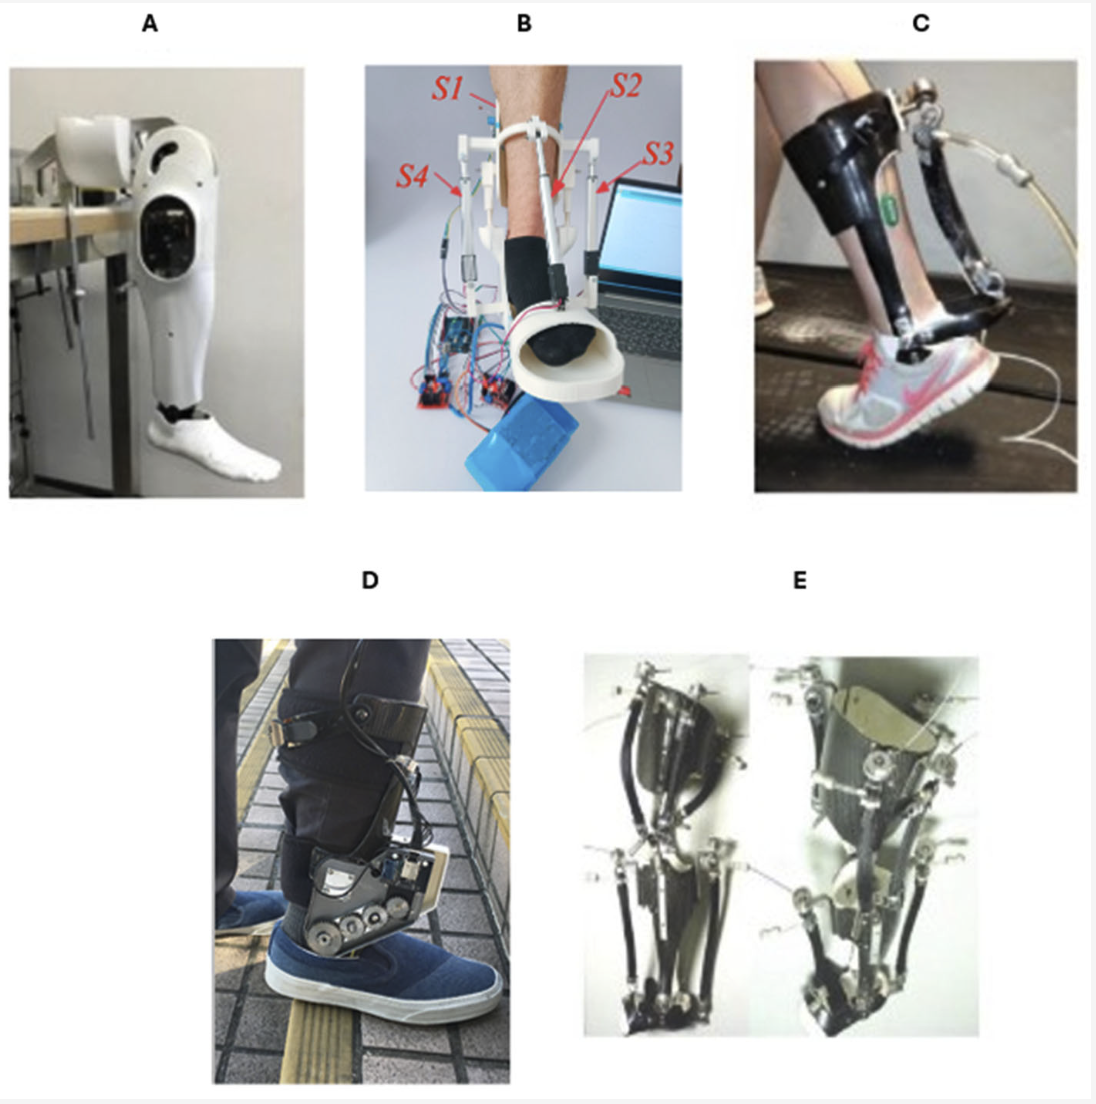
\includegraphics[width=\linewidth]{lit_exoskeletons.png}
\caption{Representative wearable ankle exoskeletons.}
\label{fig:lit-exo}
\end{subfigure}\\[0.6em]
\begin{subfigure}{0.95\linewidth}
\centering
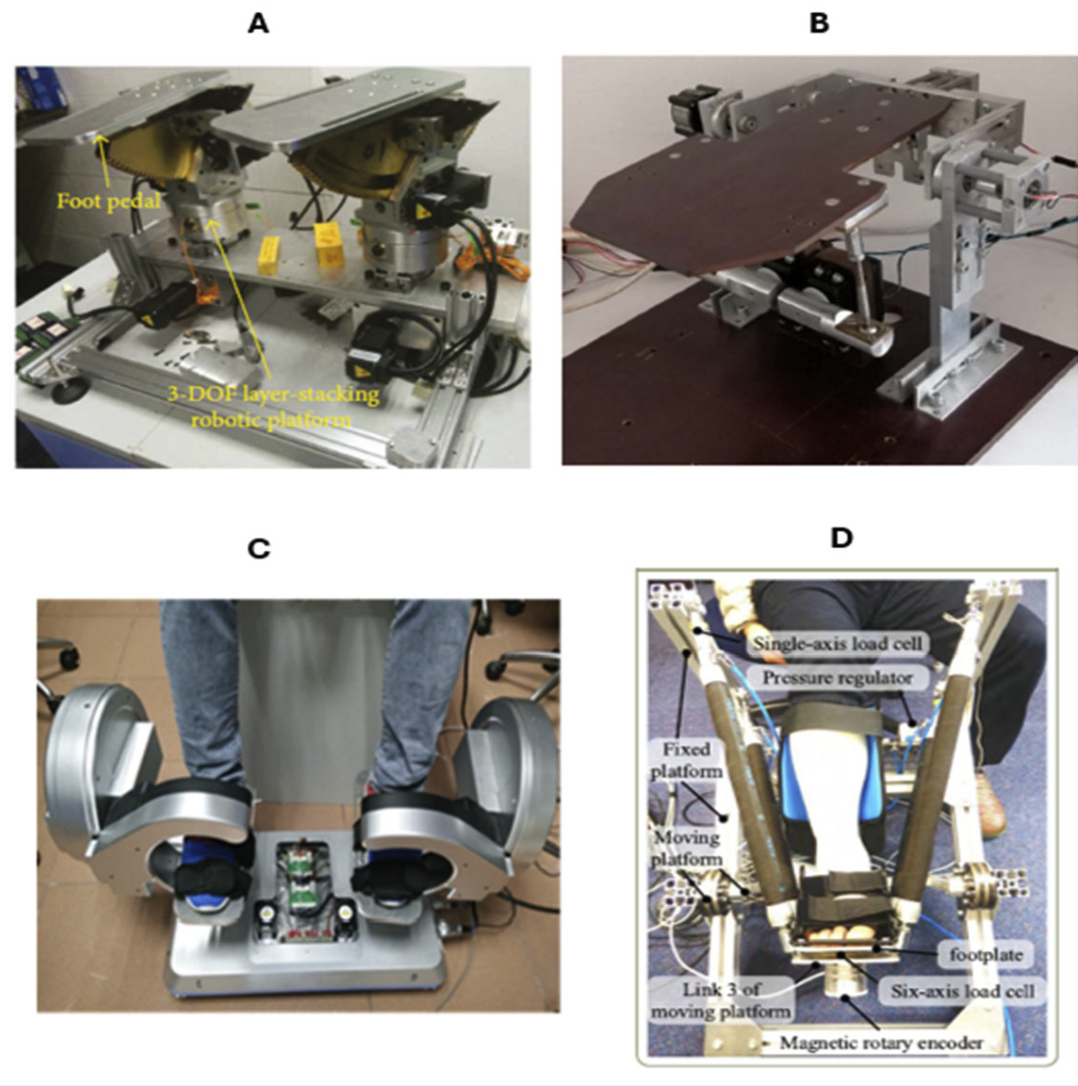
\includegraphics[width=\linewidth]{lit_platforms.png}
\caption{Representative platform-style ankle rehabilitation robots.}
\label{fig:lit-platforms}
\end{subfigure}
\caption{State of the art in ankle rehabilitation hardware. (a) Wearable exoskeletons span powered, passive, and quasi-passive designs that prioritize portability but typically constrain the joint to one or two degrees of freedom. (b) Platform-style rehabilitation devices offer multi-DOF assistance but operate in a stationary, often non-anthropomorphic frame whose center of rotation does not coincide with the talocrural joint. Our 3-RRR wearable design (Section~\ref{sec:mechanism}) targets the gap between these two families: a portable form factor that retains a remote, anatomically aligned center of rotation.}
\label{fig:literature-collage}
\end{figure}

These works converge on three design lessons. First, mass and bulk on the distal lower limb are critical: distal mass disproportionately increases the metabolic cost of walking and limits clinical adoption. Second, mechanical alignment with the biological ankle joint is essential to prevent shear loads on the talocrural complex. Third, the ability to modulate impedance, rather than to deliver a fixed trajectory, is repeatedly correlated with positive rehabilitation outcomes. Figure~\ref{fig:literature-collage} summarizes the mechanical landscape against which the proposed device is positioned.

\subsection{Spherical Parallel Mechanisms}

Parallel manipulators have a long history in robotics due to their high stiffness, accuracy, and load capacity~\cite{merlet2006jacobian}. The 3-RRR SPM is of particular interest because all of its joint axes intersect at a common point, generating three pure rotations about that point. Gosselin and Angeles~\cite{gosselin1989optimum} introduced the optimum kinematic design problem for spherical 3-DOF parallel manipulators, framed in terms of the workspace and dexterity. Saheb and Babu~\cite{saheb2021math} provided a detailed mathematical model and kinematic analysis of the planar 3-RRR architecture; their results show that the link-length ratio between the platform-side link and the base-side link directly governs the singularity distribution and the size of the singularity-free workspace. We adopt their reported optimal ratio of approximately 1.15 as the starting point for the structural-optimization study in Section~\ref{sec:mechanism}. Wu and Bai~\cite{wu2019designandkinematic} extended the analysis to a 3-RRR SPM with reconfigurable four-bar linkages, demonstrating how secondary linkages can be used to widen the dexterous workspace.

In rehabilitation, He \emph{et al.}~\cite{he2021spindle} introduced SPINDLE, a 3-RRR spherical parallel instrument designed to emulate activities of daily living for stroke rehabilitation. Sadeqi \emph{et al.}~\cite{sadeqi2017hip} analyzed a 3-RRR SPM for hip exoskeleton applications, characterizing its workspace and force-transmission performance. Both works confirm the suitability of the 3-RRR architecture for human-centered rotational tasks but operate at body locations other than the ankle. To the best of our knowledge, the only prior work that specifically targets the ankle with a 3-RRR SPM in a wearable form factor is our own~\cite{zhang2025rehab}.

\subsection{Assist-As-Needed Control and Motor Learning}

The Assist-As-Needed (AAN) paradigm, articulated by Reinkensmeyer and colleagues, posits that excessive assistance suppresses motor learning by removing the patient's incentive to contribute~\cite{cai2006implications,marchal2009review}. AAN controllers therefore aim to deliver only the minimum torque necessary to complete a desired trajectory. In practice, this requires online estimation of the patient's voluntary contribution, typically via direct force/torque sensing, electromyography~\cite{hybart2022emg}, or model-based estimation from actuator current. The latter approach is attractive for wearable devices because it eliminates the need for a distal six-axis load cell and reduces both cost and mass~\cite{zhang2015torque,jackson2019heuristic}.

Two AAN-style design considerations are particularly relevant to our system. First, the assistance gain must adapt over time. Strategies range from heuristic rules~\cite{jackson2019heuristic} that grow assistance under sustained tracking error, to model-based formulations that explicitly compute a feedforward torque from the inertial model~\cite{zhang2015torque,perez2024modeling}. Second, transparency in the absence of impairment is essential: a controller that is transparent during walking allows the user's natural gait to dominate, while AAN gains rise only when needed. Both Galle \emph{et al.}~\cite{galle2013adaptation} and Jackson and Collins~\cite{jackson2019heuristic} demonstrated that controllers that respect both criteria yield faster adaptation than fully assistive baselines.

\subsection{Wearable Sensing and Gait Analysis}

The translational value of an ankle rehabilitation robot depends as much on its sensing as on its actuation. Three sensor modalities are particularly relevant.

\emph{Inertial measurement units (IMUs)} attached to the shank and foot provide absolute orientation referenced to gravity and have become the standard tool for ambulatory gait analysis. Dual-IMU configurations enable direct estimation of ankle angle in the sagittal and frontal planes, which complements the relative joint-angle information returned by motor encoders.

\emph{Instrumented shoes and insoles} provide plantar pressure distributions and per-stride event detection. Prado \emph{et al.}~\cite{prado2020fog} demonstrated that an artificial neural network operating on instrumented-shoe signals can identify freezing of gait in Parkinson's patients, illustrating that pressure-based sensing carries clinically meaningful temporal information. Paydarfar \emph{et al.}~\cite{paydarfar2020rnn} extended this line by showing that recurrent neural networks operating on raw piezoresistive insole signals can classify human activities directly from the time series, suggesting that insoles can serve as both clinical assessment tools and real-time controller inputs. Yue \emph{et al.}~\cite{yue2018wearable} reported a wearable sensing system for lower-limb exoskeletons that combines IMU and pressure data for closed-loop control.

\emph{Gait mats and external pose tracking} provide gold-standard ground-truth data for validation. Gait mats yield stance time, swing time, step length, and the center-of-pressure (CoP) trajectory; external optical or electromagnetic trackers (such as HTC Vive trackers) supply foot-plate orientation that can be used to calibrate the kinematic model.

\emph{Cable-driven exoskeletons and post-stroke training.} Outside the ankle joint specifically, Hidayah \emph{et al.}~\cite{hidayah2020calex} reported gait adaptation results in stroke participants using a cable-driven active leg exoskeleton (C-ALEX), providing a methodological template for our AAN evaluation: a baseline walking trial, an exoskeleton-assisted training trial, and a post-training transfer trial, with quantitative gait variables (stride length, peak ankle angle, hip-knee coordination) used as outcome measures.

\subsection{Summary and Positioning}

In summary, the literature supports the following design positions, which our system adopts: (i) a parallel architecture with a fixed remote center of rotation co-located with the talocrural joint; (ii) a 3-RRR SPM optimized for an isotropic, singularity-free workspace following the link-ratio guidance of \cite{saheb2021math}; (iii) an AAN controller that uses motor current to estimate user effort and modulate assistance, in line with~\cite{cai2006implications,marchal2009review,jackson2019heuristic}; and (iv) a multi-modal sensing suite of motor encoders, dual IMUs, and a gait mat, mirroring the dual-validation approach of~\cite{hidayah2020calex,prado2020fog,yue2018wearable}.

\section{Mechanism Design and Singularity-Aware Optimization}
\label{sec:mechanism}

\subsection{Biomechanical Motivation}

The human ankle complex is biomechanically modeled as two principal joints---the talocrural and subtalar joints---whose combined motion is well approximated by three intersecting rotation axes about a single anatomical center, as illustrated in Fig.~\ref{fig:anatomy-3rrr}. The 3-RRR SPM directly mirrors this biomechanical structure: all nine revolute joints are arranged so that their axes intersect at a common spherical center $O$, generating exactly three rotational degrees of freedom about that point. The right panel of Fig.~\ref{fig:anatomy-3rrr} shows the canonical 3-RRR kinematic skeleton, with each leg comprising an actuated joint at $A_i$, a passive joint at $B_i$, and a platform connection at $C_i$ along link lengths $l_{i1}$ and $l_{i2}$.

\begin{figure}[!t]
\centering
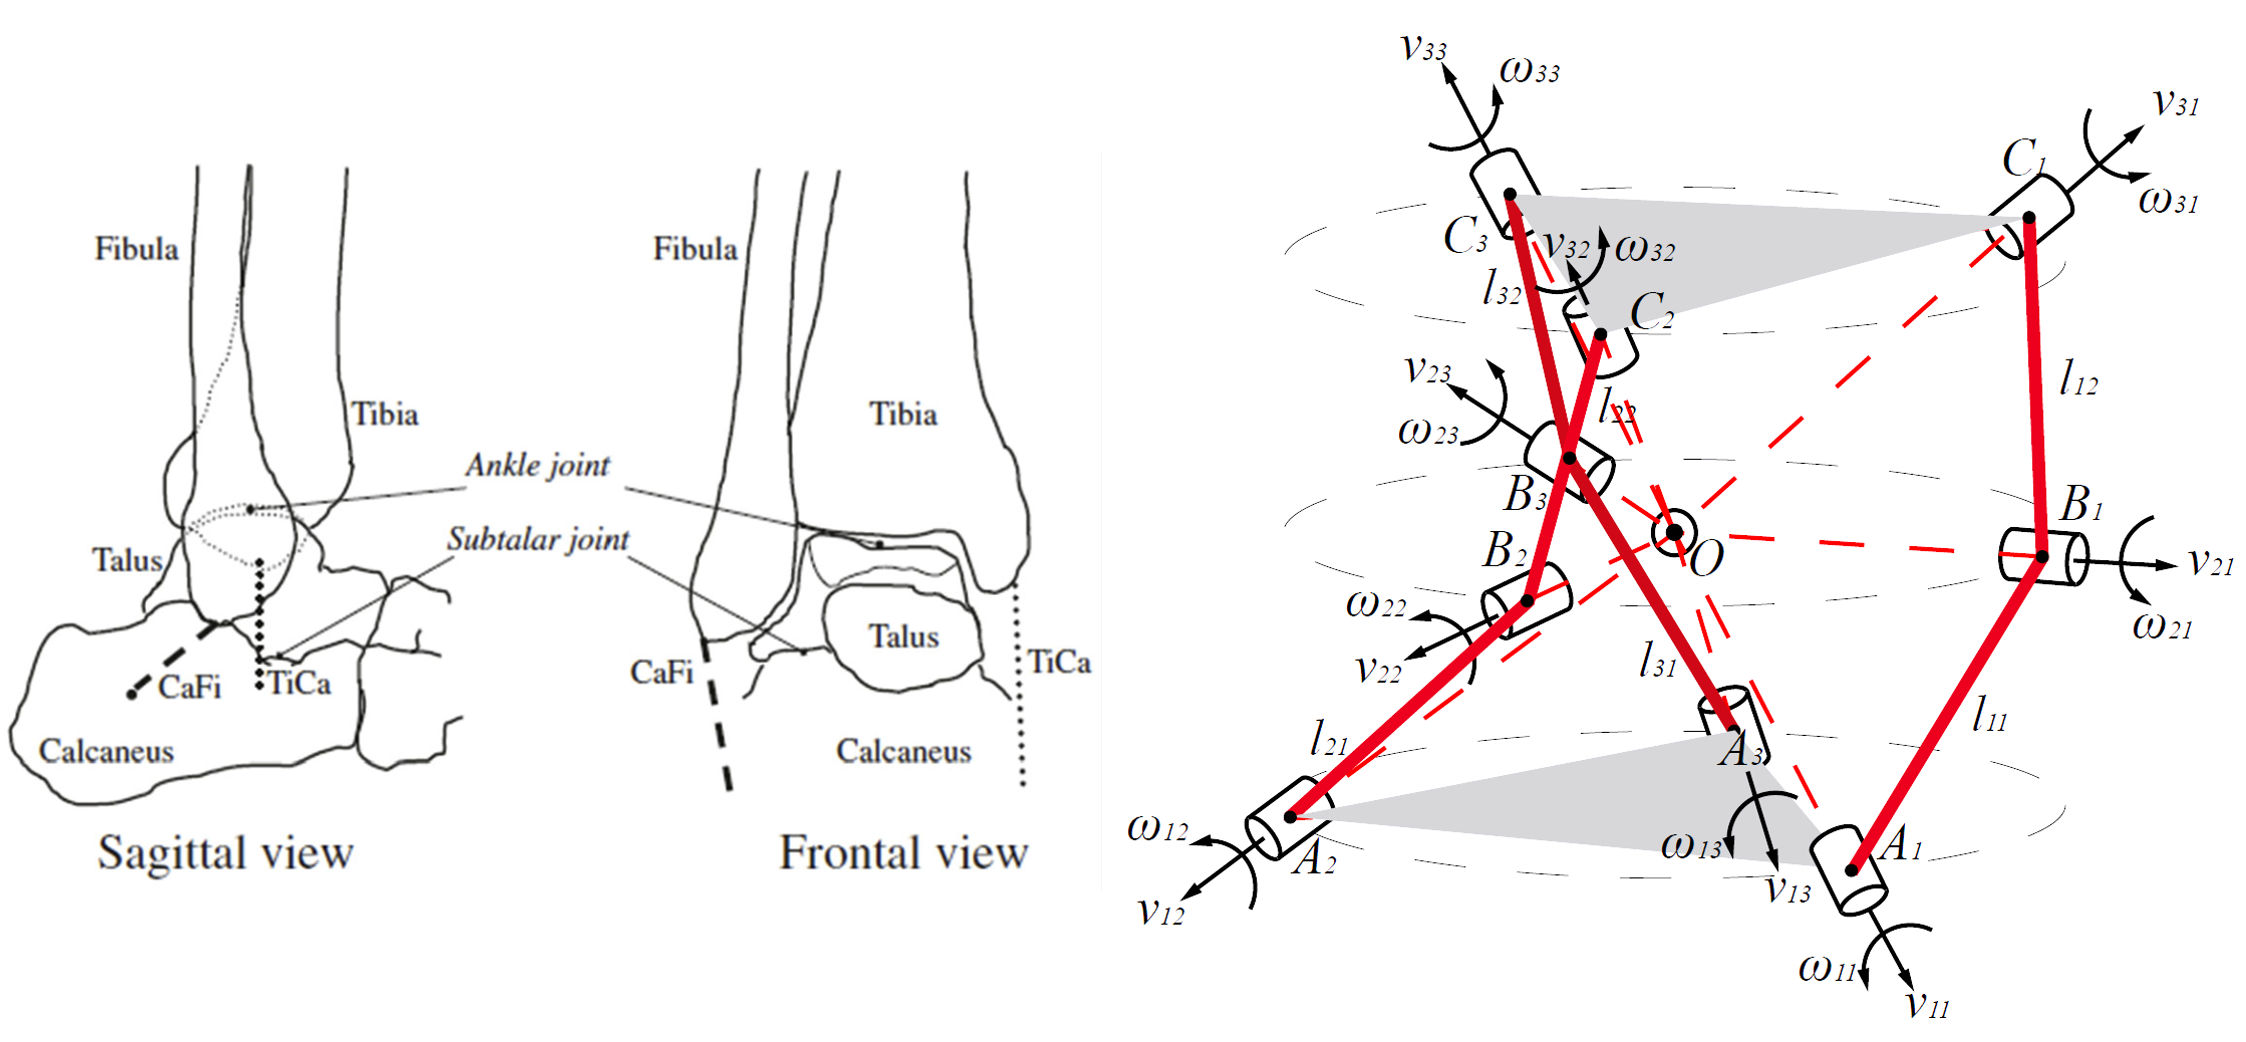
\includegraphics[width=\linewidth]{ankle_anatomy_3rrr.png}
\caption{Biomechanical motivation. \emph{Left:} sagittal and frontal anatomical views of the talocrural and subtalar complex, whose rotation axes converge near a single point. \emph{Right:} the 3-RRR spherical parallel mechanism replicates this structure: three identical limbs (each carrying actuated joint $A_i$, passive joint $B_i$, and platform connection $C_i$) intersect at a common spherical center $O$, producing exactly three rotational DOFs. Anatomical schematic adapted from the rehabilitation literature; 3-RRR diagram redrawn from kinematic conventions used in~\cite{gosselin1989optimum,saheb2021math}.}
\label{fig:anatomy-3rrr}
\end{figure}

\subsection{3-RRR Spherical Parallel Mechanism}

The proposed device consists of three identical RRR limbs that connect a ring-shaped base to a moving foot plate. Each limb contains two passive revolute joints and one actuated revolute joint at the base. All revolute axes are arranged so that they intersect at a common point, generating three rotational degrees of freedom about that point. By aligning this point with the anatomical center of the talocrural and subtalar complex during donning, the device's R-CoR is co-located with the user's H-CoR, eliminating the parasitic translations that arise from kinematic misalignment in serial or 6-DOF parallel platforms. The schematic geometry is shown in Fig.~\ref{fig:simplified-model}, where the three red kinematic chains realize the abstract architecture of Fig.~\ref{fig:anatomy-3rrr}.

\begin{figure}[!t]
\centering
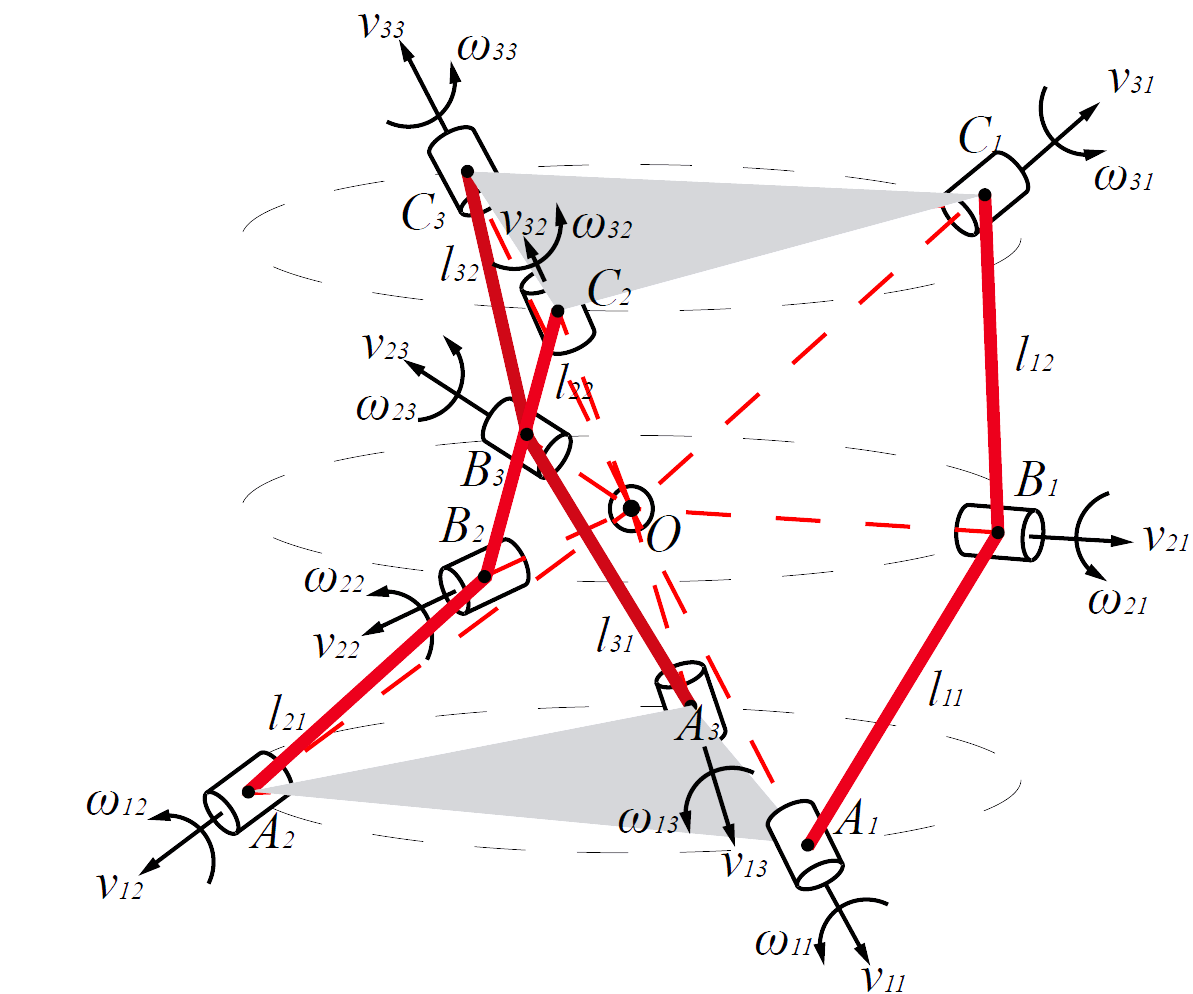
\includegraphics[width=0.78\linewidth]{simplified_model.png}
\caption{Schematic geometry of the proposed wearable 3-RRR SPM, with the ring-shaped base fixed to the shank and the moving foot plate as the end effector. The three red kinematic chains, each composed of three revolute joints and two links, realize three rotational DOFs about a common center.}
\label{fig:simplified-model}
\end{figure}

The three active joints, denoted $\theta_1$, $\theta_2$, $\theta_3$, are driven by Dynamixel XM430-W350-R smart actuators arranged at $120^{\circ}$ azimuthal spacing around the base ring. The actuators are daisy-chained over a single RS-485 bus to the master controller, providing closed-loop position, velocity, and current telemetry at high update rates~\cite{robotisxm430}.

\subsection{Wearable Embodiment}

Figure~\ref{fig:cad-prototype} shows the wearable embodiment of the mechanism that has been adopted in this project. A two-segment exoskeletal frame anchors the base ring to the shank cuff, while three actuated limbs route compactly along the medial, lateral, and posterior sides of the calf to the foot plate. Figure~\ref{fig:cad-l1l2} highlights the principal link lengths $L_1$ (proximal, base-side) and $L_2$ (distal, platform-side), which are the design parameters optimized in Section~\ref{sec:optimization} below.

\begin{figure}[!t]
\centering
\begin{subfigure}{0.31\linewidth}
\centering
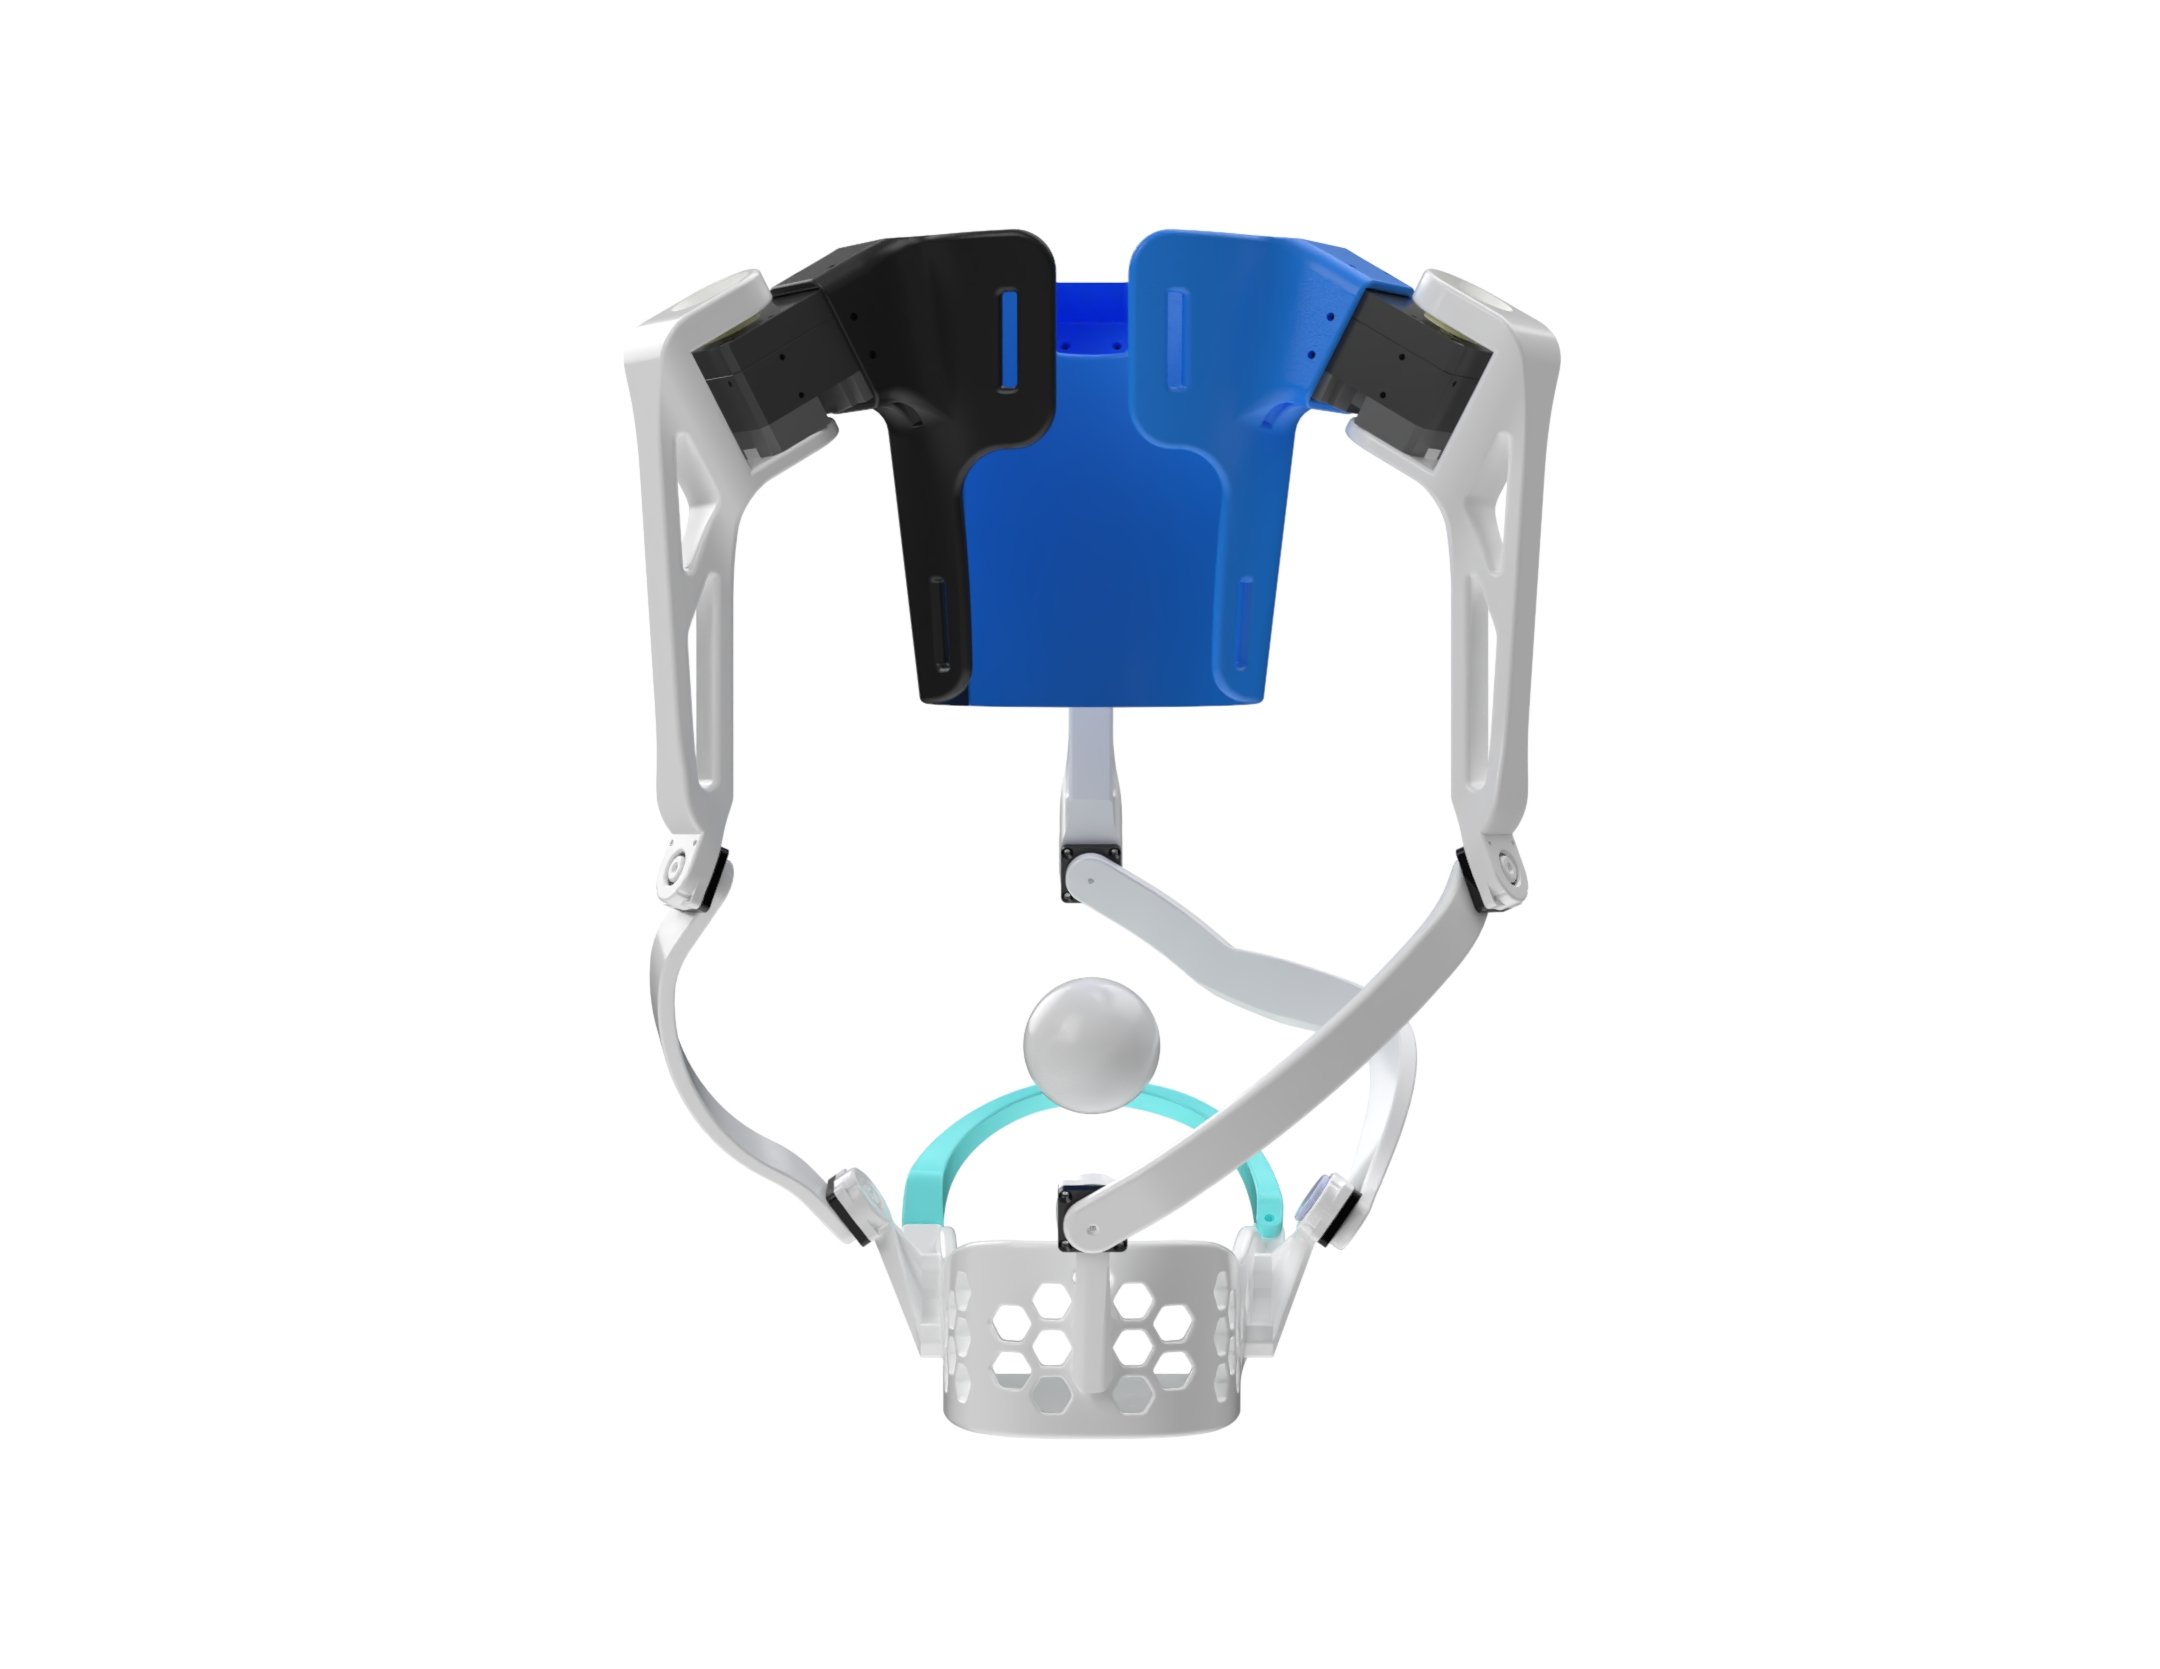
\includegraphics[width=\linewidth]{cad_front.jpg}
\caption{Front}
\label{fig:cad-front}
\end{subfigure}\hfill
\begin{subfigure}{0.31\linewidth}
\centering
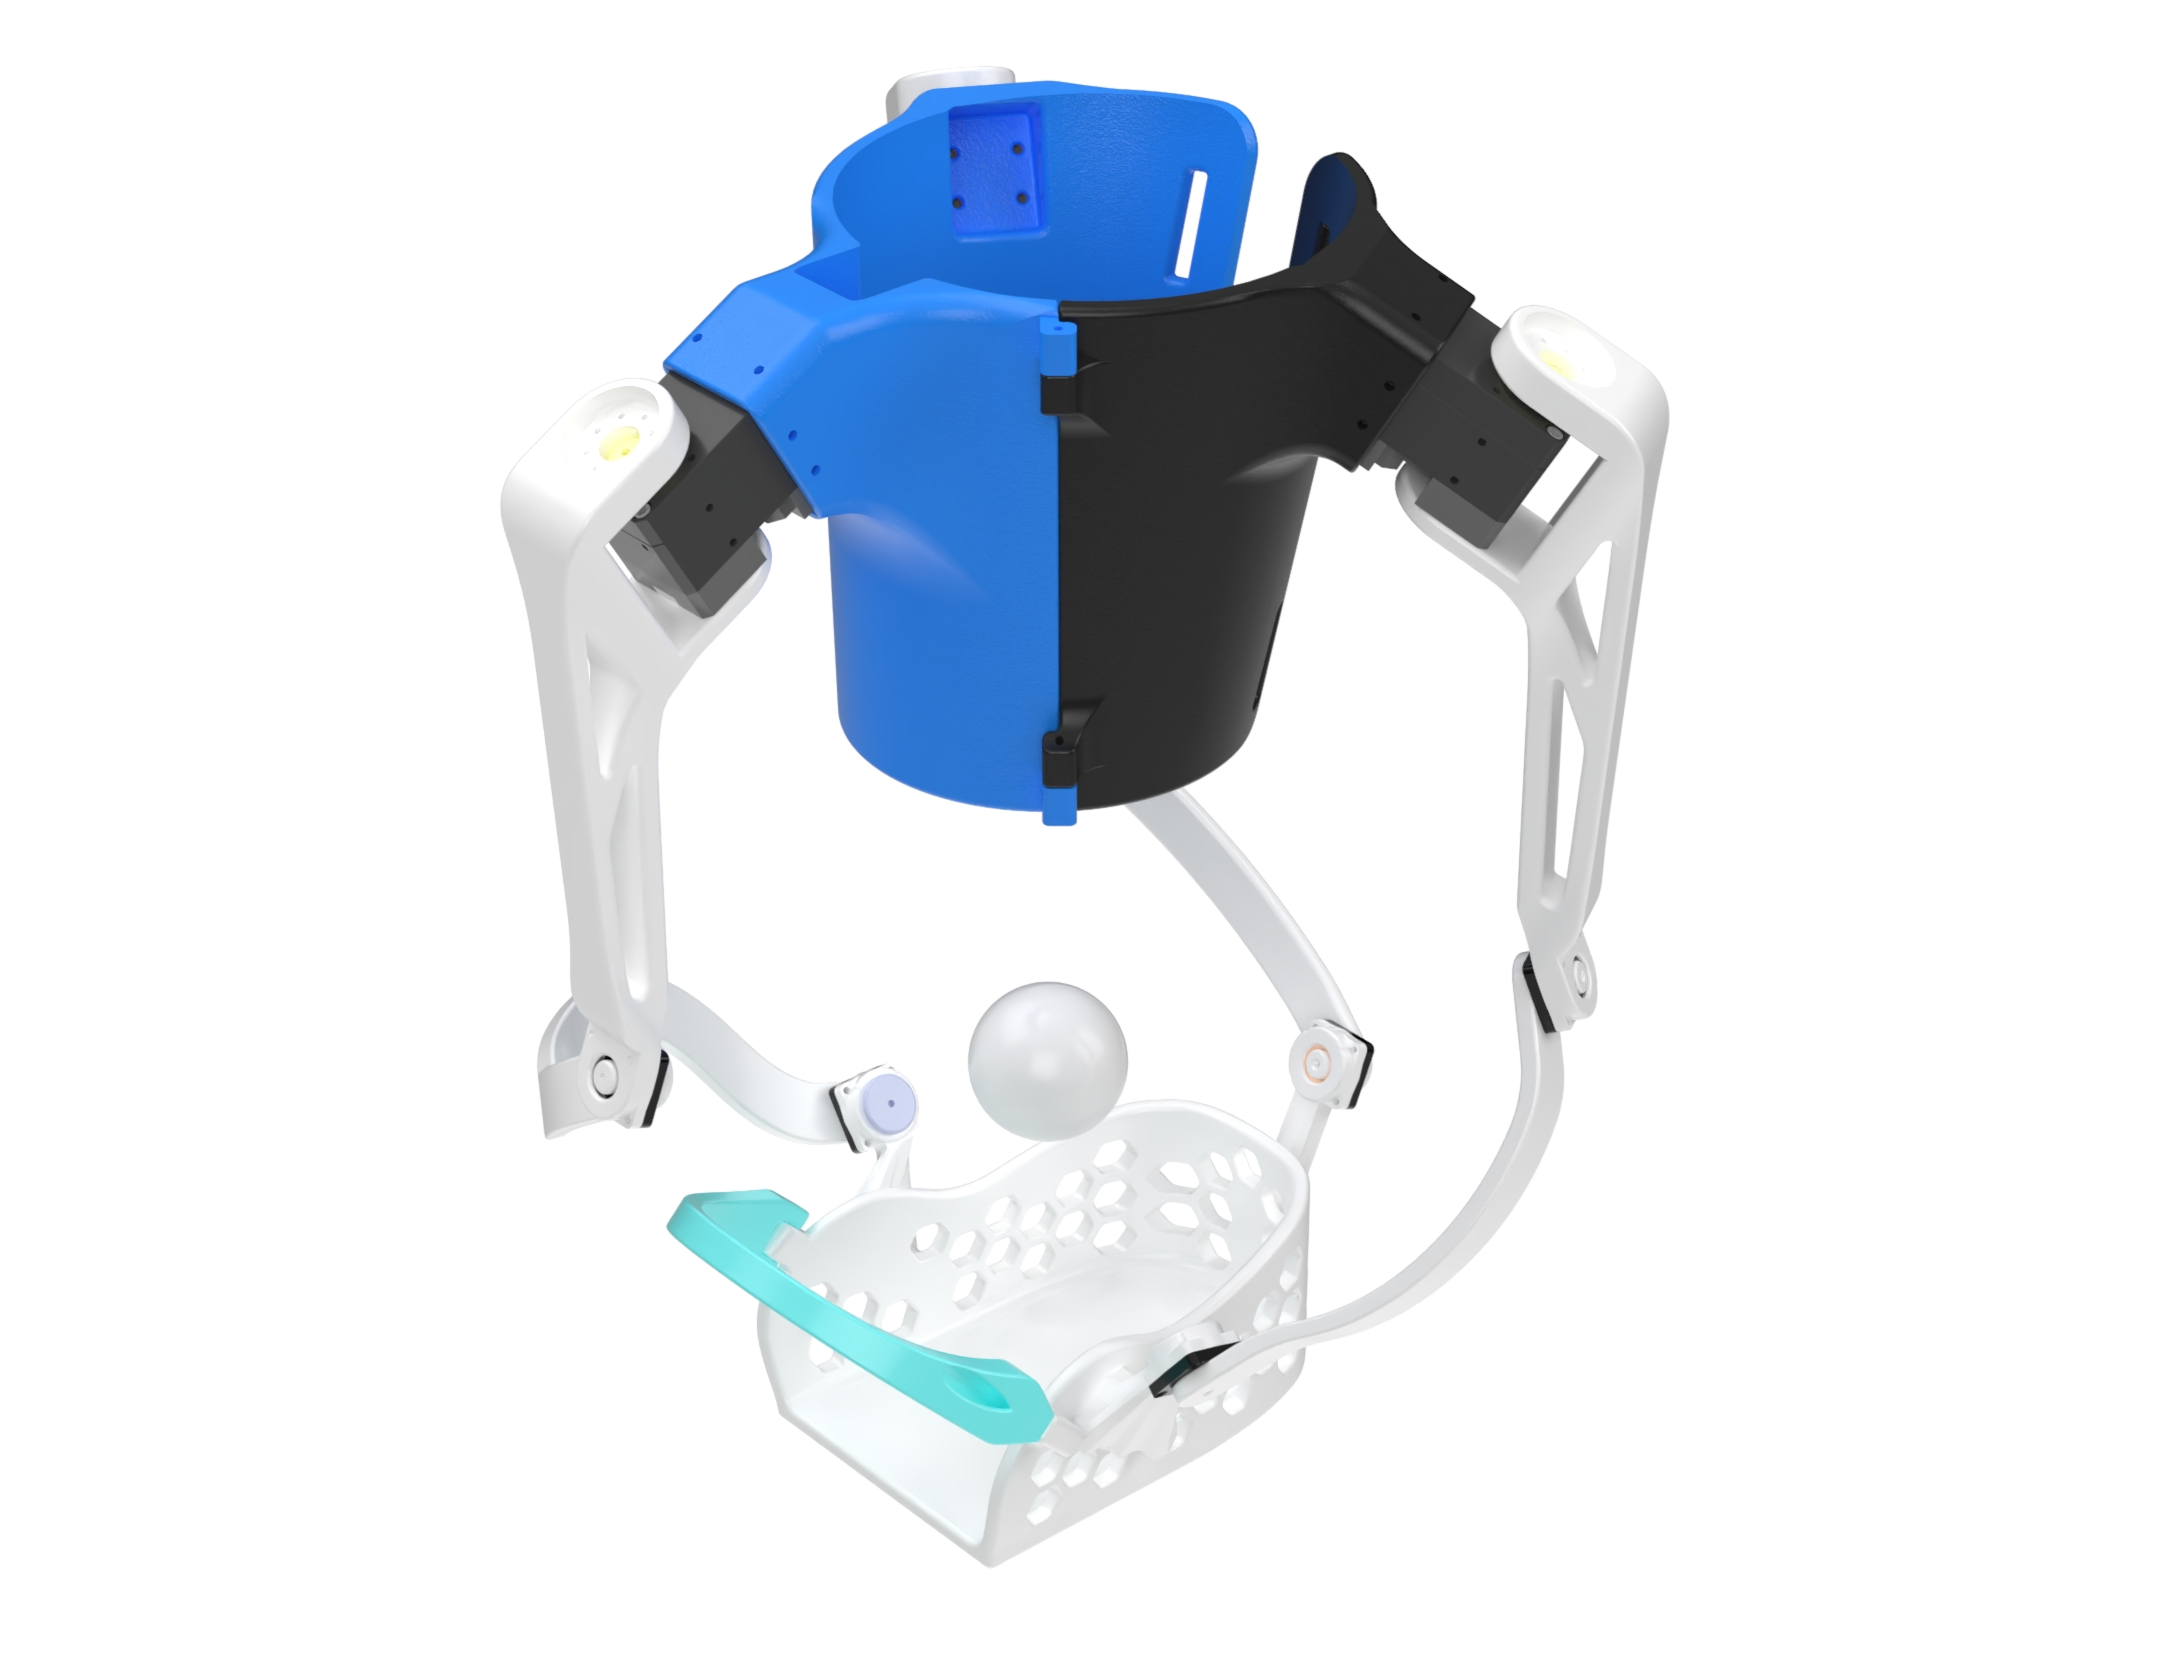
\includegraphics[width=\linewidth]{cad_perspective.jpg}
\caption{Perspective}
\label{fig:cad-pers}
\end{subfigure}\hfill
\begin{subfigure}{0.31\linewidth}
\centering
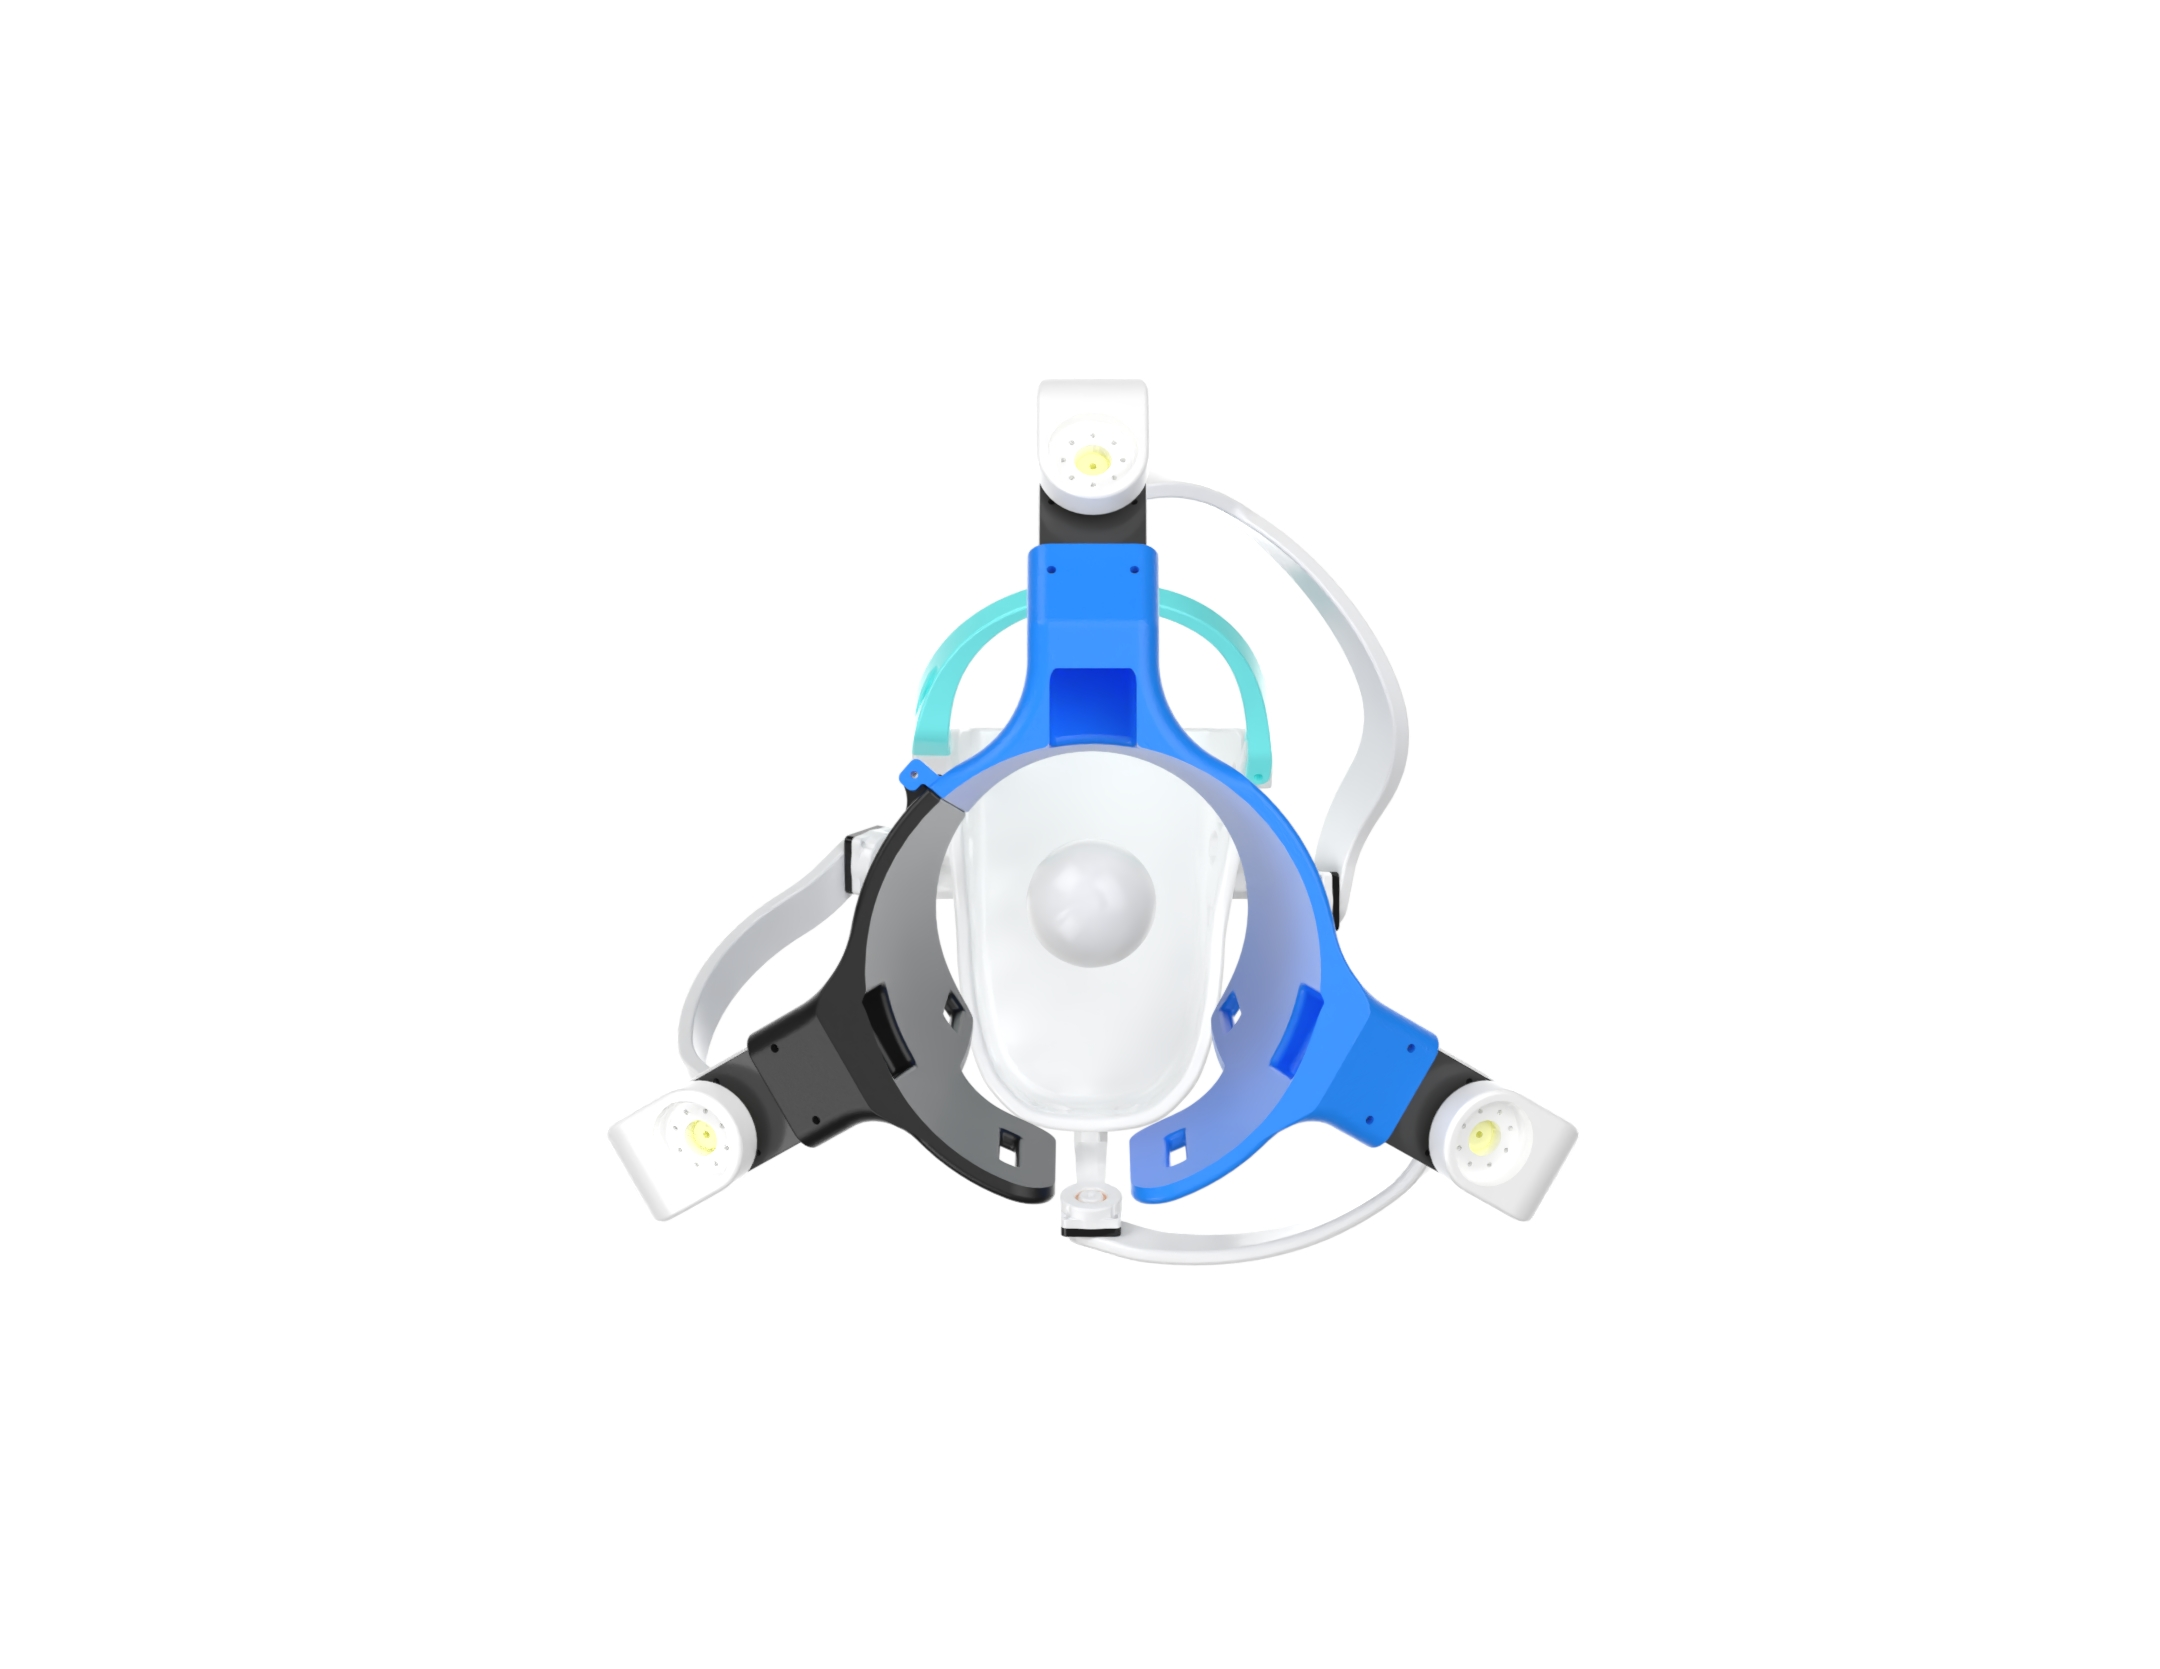
\includegraphics[width=\linewidth]{cad_top.jpg}
\caption{Top}
\label{fig:cad-top}
\end{subfigure}
\caption{Multi-view CAD renderings of the proposed wearable 3-RRR ankle rehabilitation robot. (a) Front view showing the symmetric three-limb topology around a contoured shank cuff; (b) perspective view showing the open-back base ring, distal foot plate, and the three Dynamixel housings at $120^{\circ}$ azimuthal spacing; (c) top view showing the rotational symmetry of the actuators about the spherical center.}
\label{fig:cad-prototype}
\end{figure}

\begin{figure}[!t]
\centering
\begin{subfigure}{0.46\linewidth}
\centering
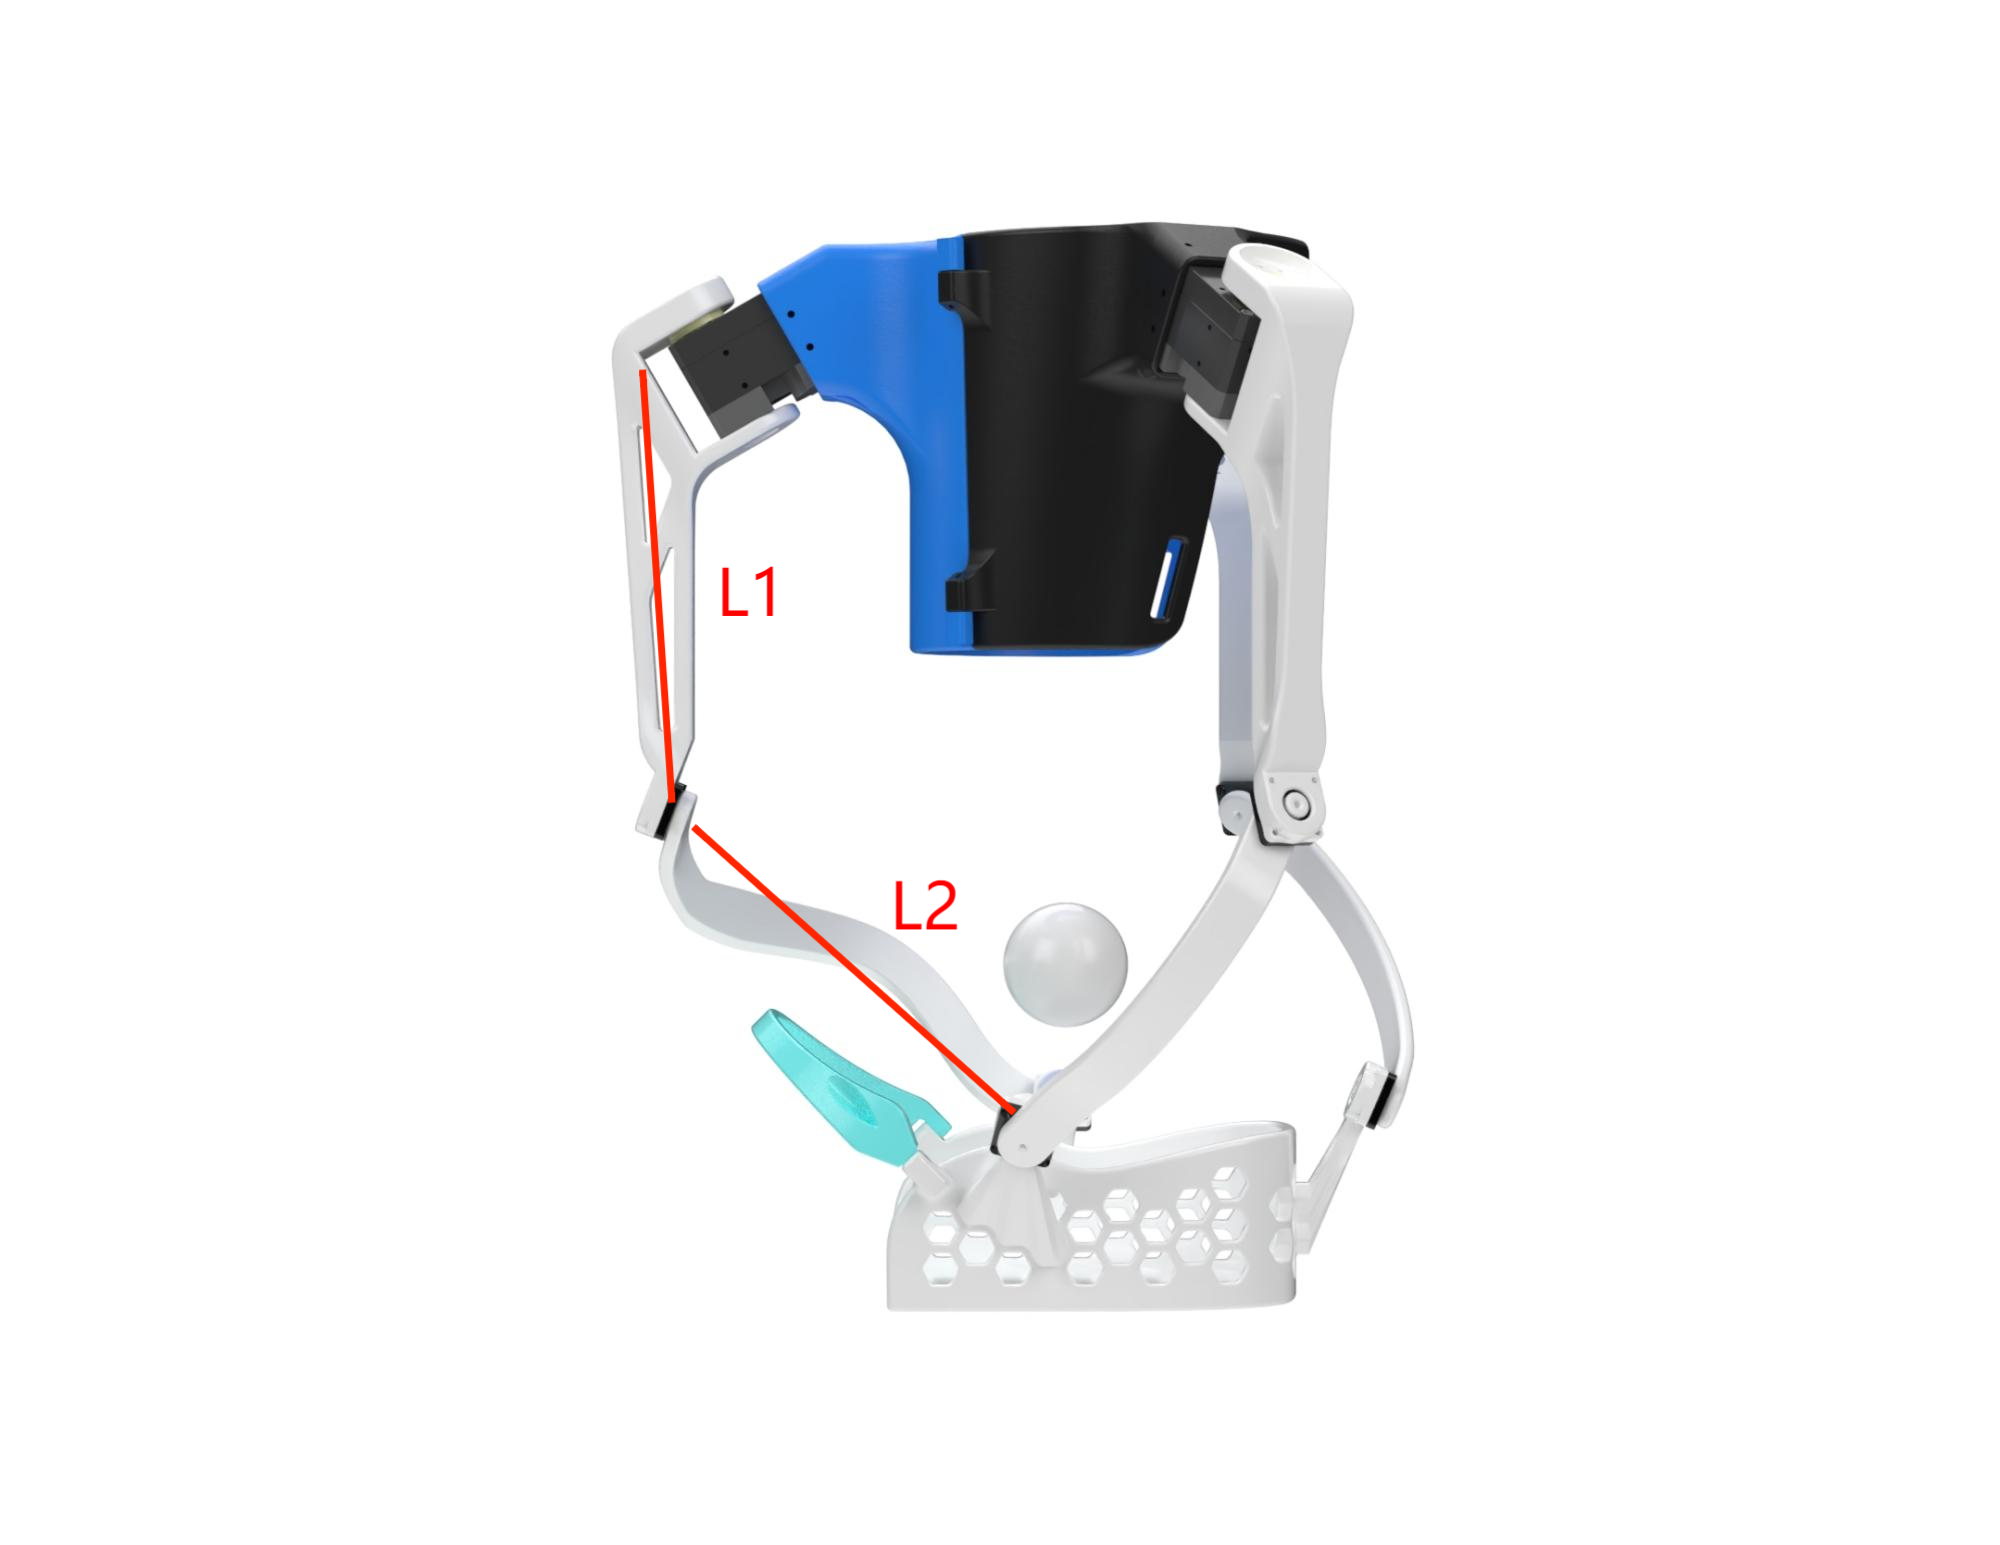
\includegraphics[width=\linewidth]{cad_l1l2.png}
\caption{CAD with link annotation}
\label{fig:cad-l1l2-cad}
\end{subfigure}\hfill
\begin{subfigure}{0.46\linewidth}
\centering
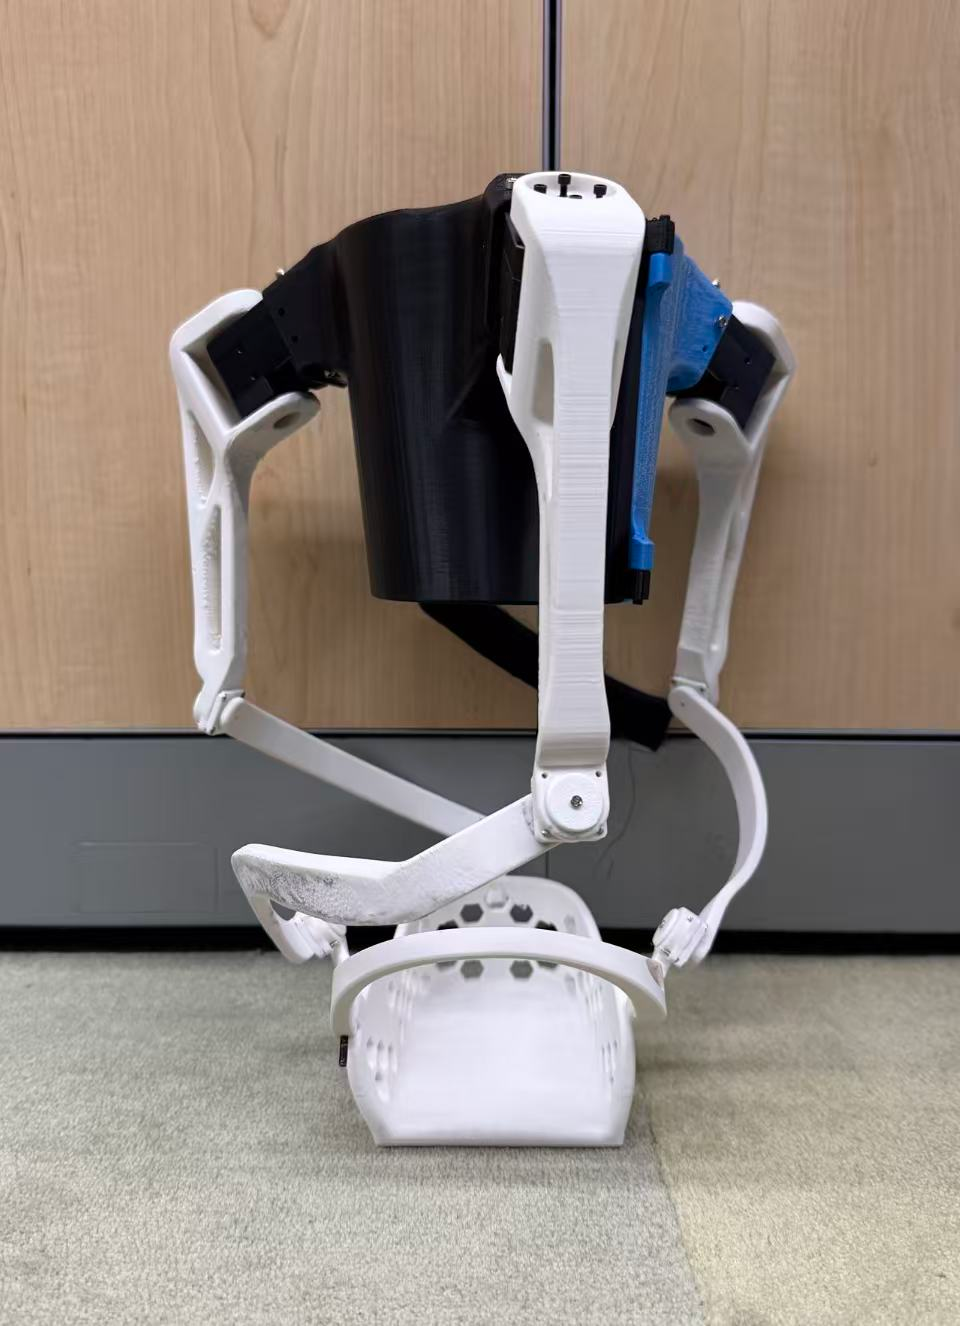
\includegraphics[width=\linewidth]{prototype_photo.png}
\caption{3D-printed prototype}
\label{fig:cad-l1l2-print}
\end{subfigure}
\caption{Wearable form factor of the 3-RRR SPM ankle rehabilitation robot. (a) Annotated CAD render highlighting the proximal link length $L_1$ (base-side) and the distal link length $L_2$ (platform-side); the design ratio $\rho=L_2/L_1$ is the principal parameter optimized in Section~\ref{sec:optimization}. (b) The 3D-printed prototype that has been used for static fitting, range-of-motion verification, and as the integration platform for the embedded control hardware described in Section~\ref{sec:hardware}.}
\label{fig:cad-l1l2}
\end{figure}

The wearable form factor introduces several engineering constraints that informed the design:
\begin{itemize}
\item a compact base ring with adjustable straps for secure, comfortable attachment;
\item non-interfering limb routing to avoid contact with adjacent anatomy, footwear, and orthotic braces;
\item modular interchangeable links and quick-release fasteners that support adaptation across users and rehabilitation stages.
\end{itemize}

\subsection{Parallel Singularities and the Need for Geometric Optimization}

A central challenge of any parallel mechanism is the existence of \emph{parallel singularities}, configurations at which the moving platform gains uncontrollable instantaneous degrees of freedom even when all actuators are locked~\cite{merlet2006jacobian}. In a rehabilitation context, this is both a control concern and a safety concern: at a parallel singularity, the device loses stiffness and can no longer resist external loads transmitted through the patient's foot.

In the constraint formulation, the relationship between the platform angular velocity $\boldsymbol{\omega}\in\mathbb{R}^3$ and the active-joint rate $\dot{\boldsymbol{q}}\in\mathbb{R}^3$ is
\begin{equation}
\mathbf{A}\,\boldsymbol{\omega}+\mathbf{B}\,\dot{\boldsymbol{q}}=\mathbf{0},
\label{eq:constraint}
\end{equation}
where $\mathbf{A}$ is the constraint Jacobian and $\mathbf{B}$ is the actuation Jacobian. Type-2 (parallel) singularities occur when $\det(\mathbf{A})\to 0$. In our prior design~\cite{zhang2025rehab}, candidate singular configurations were identified by numerically tracking $\det(\mathbf{A})$ over the workspace, and avoidance was achieved by mechanically restricting each active joint to a conservative range. While effective, this approach is inherently reactive: it \emph{avoids} singular regions rather than removing them.

\subsection{Link-Ratio Optimization}
\label{sec:optimization}

Following the analytical framework of Saheb and Babu~\cite{saheb2021math} and the parametric study of Wu and Bai~\cite{wu2019designandkinematic}, two design parameters dominate isotropy and singularity placement in the 3-RRR architecture:
\begin{itemize}
\item the proximal (base-side) link length $l_1$, and
\item the distal (platform-side) link length $l_2$, with the design ratio $\rho=l_2/l_1$.
\end{itemize}
The reported optimum for a wide range of 3-RRR designs lies near
\begin{equation}
\rho=\frac{l_2}{l_1}\approx 1.15,
\label{eq:rho}
\end{equation}
at which the global isotropy index, computed as the mean inverse condition number of the rotational Jacobian over a discretized workspace, is maximized and the singular curves are pushed toward the boundary of the workspace. We adopted $\rho\approx 1.15$ as our design ratio and re-computed the singularity distribution; the resulting reachable workspace projected onto the platform-rotation plane is shown in Fig.~\ref{fig:workspace}. The three intersecting circular regions correspond to the per-leg reachable sets, whose intersection is the parallel-singularity-free common workspace. The blue markers denote the platform connection points $\mathbf{C}_i$ in the home pose. We observed three quantitative improvements relative to the prior design~\cite{zhang2025rehab}:
\begin{enumerate}
\item the mean isotropy index improved by approximately \textbf{20\%};
\item interior singular regions were compressed toward the workspace boundary;
\item the safe usable workspace, defined as the set of poses with condition number below a fixed threshold, expanded measurably.
\end{enumerate}
The device therefore reduces singular behavior at the structural level rather than relying solely on motor-side joint-limit avoidance. The remaining motor-side limits in Section~\ref{sec:hardware} are imposed for patient safety, not for singularity avoidance.

\begin{figure}[!t]
\centering
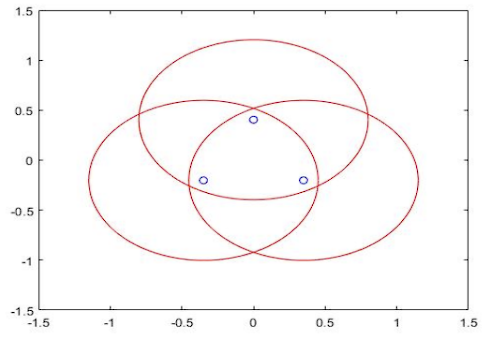
\includegraphics[width=0.78\linewidth]{workspace_plot.png}
\caption{Per-leg reachable regions and the common rotational workspace of the optimized 3-RRR mechanism, projected onto the platform-rotation plane. Each red circle is the locus reachable by one leg's distal endpoint $\mathbf{C}_i$ as $\theta_i$ sweeps through its admissible range; their intersection is the parallel-singularity-free common workspace. Blue markers denote the platform connection points in the neutral pose. The optimized link ratio $\rho\approx 1.15$ enlarges this intersection and pushes singular curves outward toward the boundary.}
\label{fig:workspace}
\end{figure}

\section{Kinematic Modeling}
\label{sec:kinematics}

\subsection{Notation and Reference Frames}

For each leg $i\in\{1,2,3\}$, we define the points listed in Table~\ref{tab:notation}, all expressed in a fixed base frame $\{B\}$ centered at the spherical center of rotation $C$. The neutral foot-plate frame $\{F\}$ is rigidly attached to the moving foot plate. A foot-plate point with coordinates $\mathbf{p}_i^F$ in $\{F\}$ has base-frame coordinates
\begin{equation}
\mathbf{C}_i^B = \mathbf{C}_B + R_{BF}\,\mathbf{p}_i^F,
\label{eq:platform-point}
\end{equation}
where the foot-plate orientation is parameterized using clinically meaningful Euler angles
\begin{equation}
R_{BF} = R_z(\mathrm{yaw})\,R_y(\mathrm{pitch})\,R_x(\mathrm{roll}).
\label{eq:rbf}
\end{equation}

\begin{table}[!t]
\centering
\caption{Geometric notation for leg $i$.}
\label{tab:notation}
\begin{tabular}{cl}
\toprule
\textbf{Symbol} & \textbf{Description}\\
\midrule
$\mathbf{A}_i$ & Actuated base-joint center\\
$\mathbf{B}_i$ & Intermediate (passive) joint center\\
$\mathbf{C}_i$ & Platform connection point of leg $i$\\
$\mathbf{u}_i$ & Unit direction of the active motor axis\\
$P$            & Platform center / spherical center\\
$l_1$          & Length of proximal link $\overline{\mathbf{A}_i\mathbf{B}_i}$\\
$l_2$          & Length of distal link  $\overline{\mathbf{B}_i\mathbf{C}_i}$\\
$\theta_i$     & Active joint angle of leg $i$\\
\bottomrule
\end{tabular}
\end{table}

\subsection{Closed-Form Inverse Kinematics}

Given a desired pose $(\mathrm{roll},\,\mathrm{pitch},\,\mathrm{yaw})$, each platform-side point $\mathbf{C}_i$ is computed from \eqref{eq:platform-point}--\eqref{eq:rbf}. Each leg must then satisfy the two link-length constraints
\begin{equation}
\|\mathbf{B}_i-\mathbf{A}_i\|=l_1,\qquad
\|\mathbf{C}_i-\mathbf{B}_i\|=l_2.
\label{eq:linkconstraints}
\end{equation}
Letting $d=\|\mathbf{C}_i-\mathbf{A}_i\|$, the projection ratio along the chord and the perpendicular offset are
\begin{equation}
\eta=\frac{l_1^2-l_2^2+d^2}{2d^2},\qquad
\xi=\sqrt{l_1^2-(\eta d)^2}.
\end{equation}
The intermediate joint center is
\begin{equation}
\mathbf{B}_i=\mathbf{A}_i+\eta\,(\mathbf{C}_i-\mathbf{A}_i)+\xi\,\frac{(\mathbf{C}_i-\mathbf{A}_i)\times \mathbf{N}}{\|(\mathbf{C}_i-\mathbf{A}_i)\times \mathbf{N}\|},
\end{equation}
where $\mathbf{N}$ is a leg-specific normal vector that selects the assembly mode. The active angle is finally extracted by projecting $\mathbf{B}_i-\mathbf{A}_i$ onto the motor-axis direction $\mathbf{u}_i$:
\begin{equation}
\theta_i=\cos^{-1}\!\left(\frac{(\mathbf{B}_i-\mathbf{A}_i)\cdot \mathbf{u}_i}{\|\mathbf{B}_i-\mathbf{A}_i\|}\right).
\label{eq:active-angle}
\end{equation}
The closed-form expression \eqref{eq:active-angle} is well-suited for offline workspace evaluation and trajectory pre-computation.

\subsection{Numerical Inverse Kinematics for Real-Time Control}

For real-time control, we model each leg as one effective rigid link of length $L_i$ between an actuator-side horn point and a foot-plate point. With motor angle $q_i$, the actuator-side point is
\begin{equation}
\mathbf{A}_i^B(q_i)=\mathbf{B}_i^B+\mathrm{Rot}(\mathbf{u}_i^B,\,q_i-q_{i0})\,(\mathbf{A}_{i0}^B-\mathbf{B}_i^B),
\end{equation}
where $\mathbf{B}_i^B$ is the motor-axis pivot point, $\mathbf{u}_i^B$ is the motor axis, and $q_{i0}$ is the motor zero offset. The leg constraint reduces to a scalar equation
\begin{equation}
f_i(q_i)=\|\mathbf{P}_i^B-\mathbf{A}_i^B(q_i)\|-L_i=0.
\label{eq:leg-constraint}
\end{equation}
A bracket-and-bisection root finder solves \eqref{eq:leg-constraint} on each control cycle. When multiple solutions exist, the solver selects the root closest to the previous time step to enforce branch continuity, which is essential to prevent discontinuous motor commands during real-time operation.

\subsection{Velocity Kinematics and Conditioning}

Under pure rotation about the spherical center, $\dot{\mathbf{P}}=\mathbf{0}$, the velocity of $\mathbf{B}_i$ is $\mathbf{v}_{B_i}=\boldsymbol{\omega}\times\mathbf{r}_i$, with $\mathbf{r}_i=\mathbf{B}_i-P$. Defining $\mathbf{L}_i$ as the unit vector from $\mathbf{B}_i$ to $\mathbf{C}_i$, the active-joint rate satisfies $\dot{\theta}_i=\mathbf{L}_i^{\!T}(\boldsymbol{\omega}\times\mathbf{r}_i)=(\mathbf{r}_i\times\mathbf{L}_i)^{\!T}\boldsymbol{\omega}$. Stacking three legs yields the rotational Jacobian
\begin{equation}
\dot{\boldsymbol{q}}=\mathbf{J}_r\,\boldsymbol{\omega},\quad
\mathbf{J}_r=\begin{bmatrix}(\mathbf{r}_1\times\mathbf{L}_1)^{\!T}\\(\mathbf{r}_2\times\mathbf{L}_2)^{\!T}\\(\mathbf{r}_3\times\mathbf{L}_3)^{\!T}\end{bmatrix}.
\label{eq:jacobian}
\end{equation}
The conditioning of $\mathbf{J}_r$, measured by its condition number $\kappa(\mathbf{J}_r)$, is exactly the quantity improved by the structural optimization of Section~\ref{sec:mechanism}. A well-conditioned $\mathbf{J}_r$ avoids motor-torque blow-up near singularities and permits a uniform mapping between platform velocity and motor velocity. The condition number is also monitored online by the safety supervisor (Section~\ref{sec:hardware}) and used to limit commanded velocities near the workspace boundary.

\section{Dynamics and Baseline Control}
\label{sec:dynamics}

\subsection{Lagrangian Model}

Following~\cite{zhang2025rehab}, we adopt the actuated joint angles $\boldsymbol{q}=[\theta_1,\theta_2,\theta_3]^{\!T}$ as generalized coordinates. The kinetic energy combines the platform's rotational energy with the limb-side rotational energy:
\begin{equation}
T=\tfrac{1}{2}\boldsymbol{\omega}^{\!T}I_P\boldsymbol{\omega}+\tfrac{1}{2}\sum_{i=1}^3 I_{\ell,i}\dot{\theta}_i^2.
\end{equation}
Because all rigid-body centers of mass rotate about a fixed point (the spherical center) and the moving foot plate is approximately balanced, the gravitational potential energy contribution is small, $V\approx 0$, and the gravity vector $G(\boldsymbol{q})\approx\mathbf{0}$. Applying Lagrange's equations and substituting $\boldsymbol{\omega}=\mathbf{J}_r^{+}\dot{\boldsymbol{q}}$ yields the rigid-body equations of motion
\begin{equation}
M(\boldsymbol{q})\ddot{\boldsymbol{q}}+C(\boldsymbol{q},\dot{\boldsymbol{q}})\dot{\boldsymbol{q}}=\boldsymbol{\tau}_{\mathrm{motor}}+\boldsymbol{\tau}_{\mathrm{ext}},
\label{eq:dynamics}
\end{equation}
with $M(\boldsymbol{q})=\mathbf{J}_r^{+T}I_P\mathbf{J}_r^{+}+\mathrm{diag}(I_{\ell,1},I_{\ell,2},I_{\ell,3})$, the standard Christoffel form for $C(\boldsymbol{q},\dot{\boldsymbol{q}})$, and $\boldsymbol{\tau}_{\mathrm{ext}}$ representing the external torque applied by the patient's foot.

\subsection{PID Baseline}

A baseline reference controller is provided by three independent PID loops on the actuator angles:
\begin{equation}
\tau_{\mathrm{motor},i}(t)=K_{p,i}\,e_i(t)+K_{d,i}\,\dot{e}_i(t)+K_{i,i}\!\int_0^t\!e_i(\sigma)\,d\sigma,
\label{eq:pid}
\end{equation}
with $e_i=q_{i,\mathrm{ref}}-q_i$. Two tunings were explored in our prior work~\cite{zhang2025rehab}: an underdamped tuning $(K_p,K_d,K_i)=(20,0.5,1)$ that emulates a high-compliance interaction, and a critically damped tuning $(K_p,K_d,K_i)=(50,2,5)$ intended for fast monotonic tracking. Figure~\ref{fig:pid-baseline} shows the resulting platform orientation responses to a step reference of $[15^{\circ},10^{\circ},5^{\circ}]^{\!T}$ in (roll, pitch, yaw). The underdamped controller (Fig.~\ref{fig:pid-under}) exhibits sustained oscillations around the target due to low damping, whereas the critically damped controller (Fig.~\ref{fig:pid-crit}) converges monotonically without overshoot. The qualitative result is that even on a rigid SPM, the choice of feedback gain modulates effective compliance. This insight is the foundation for the AAN strategy in Section~\ref{sec:aan}, which dynamically blends a feedforward inverse-dynamics term with a tunable feedback term to produce variable assistance.

\begin{figure}[!t]
\centering
\begin{subfigure}{0.95\linewidth}
\centering
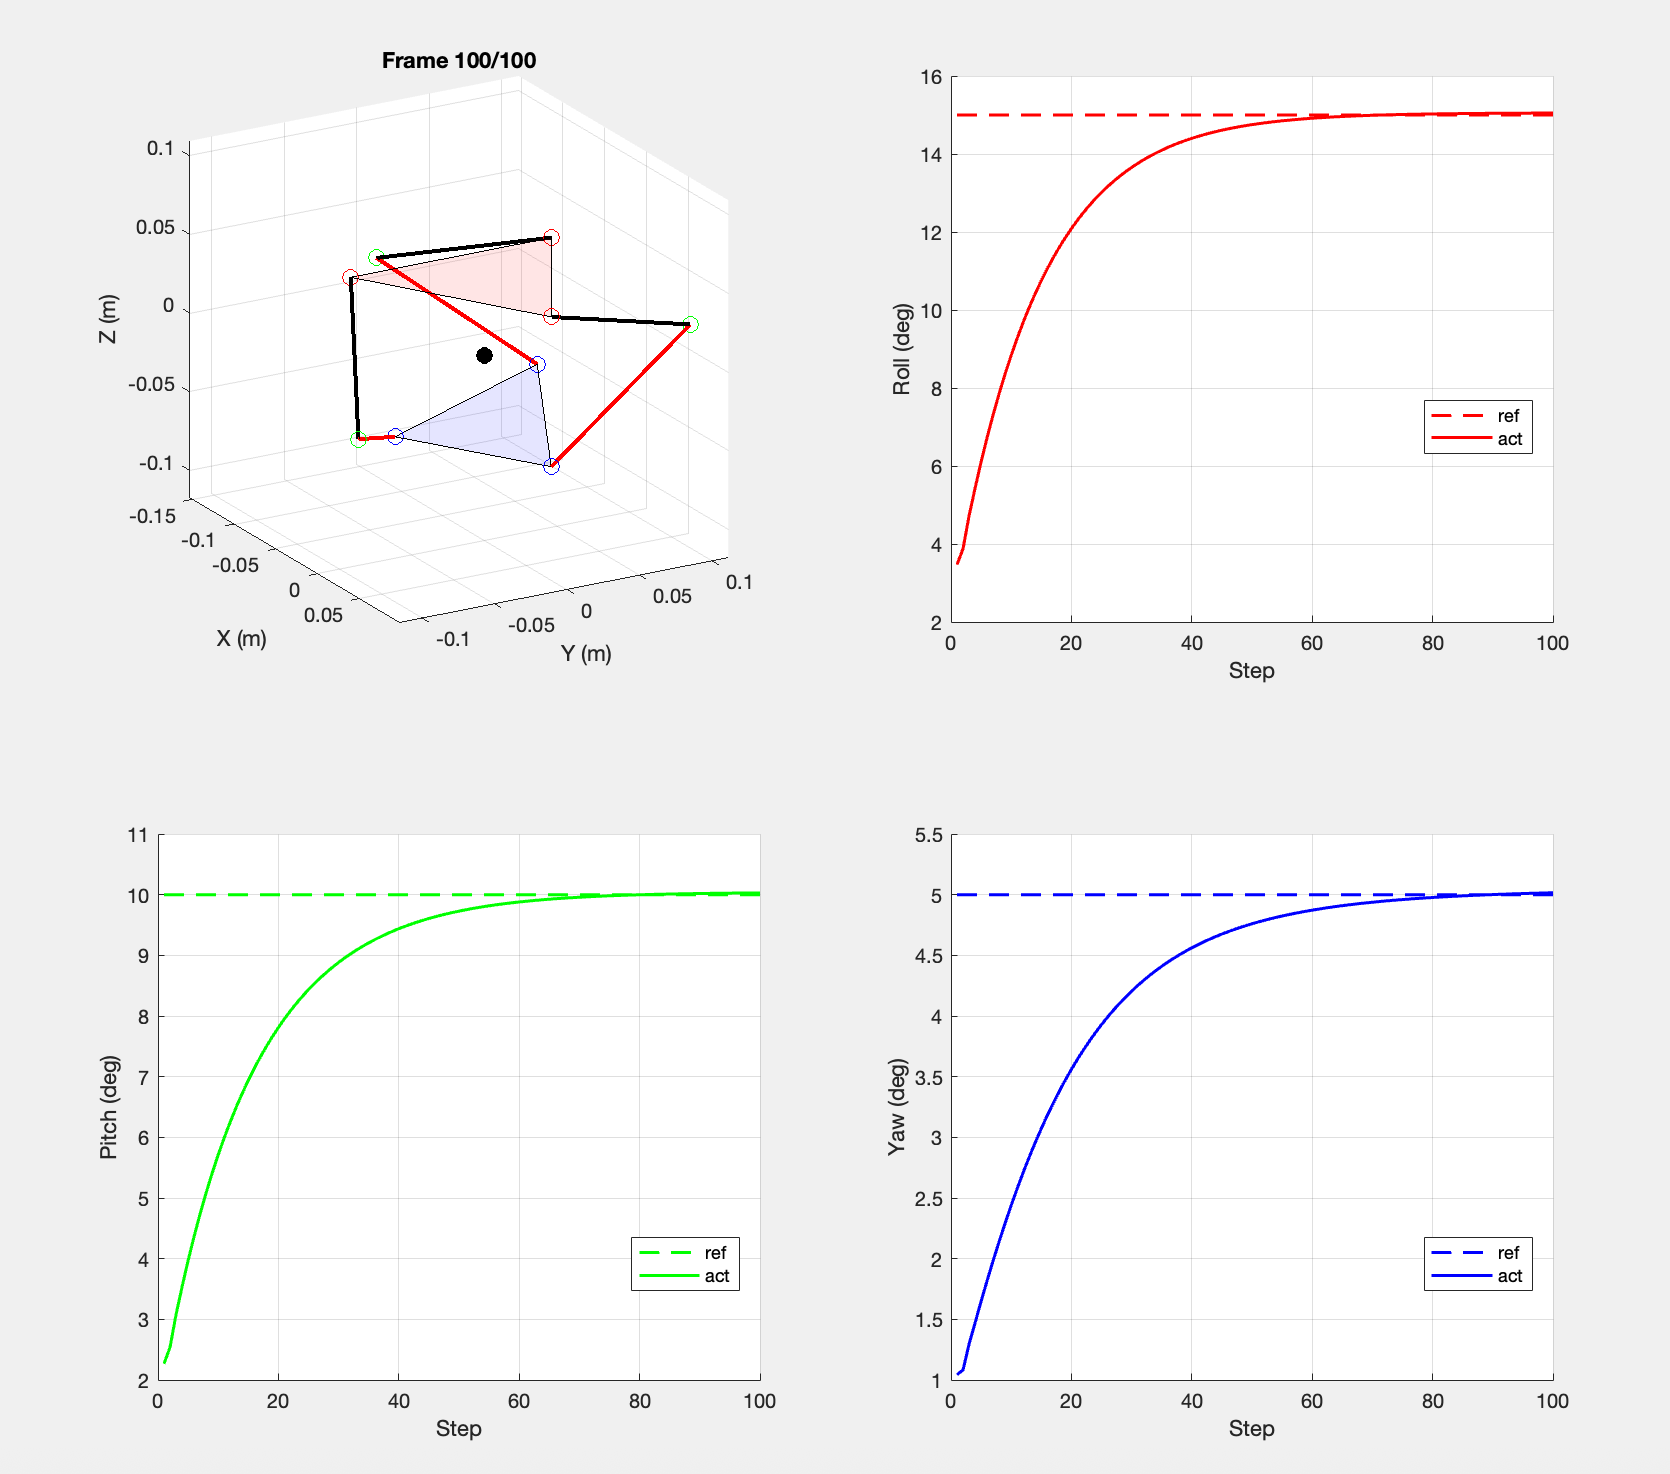
\includegraphics[width=\linewidth]{underdamped_response.png}
\caption{Underdamped tuning $(K_p,K_d,K_i)=(20,0.5,1)$.}
\label{fig:pid-under}
\end{subfigure}\\[0.4em]
\begin{subfigure}{0.95\linewidth}
\centering
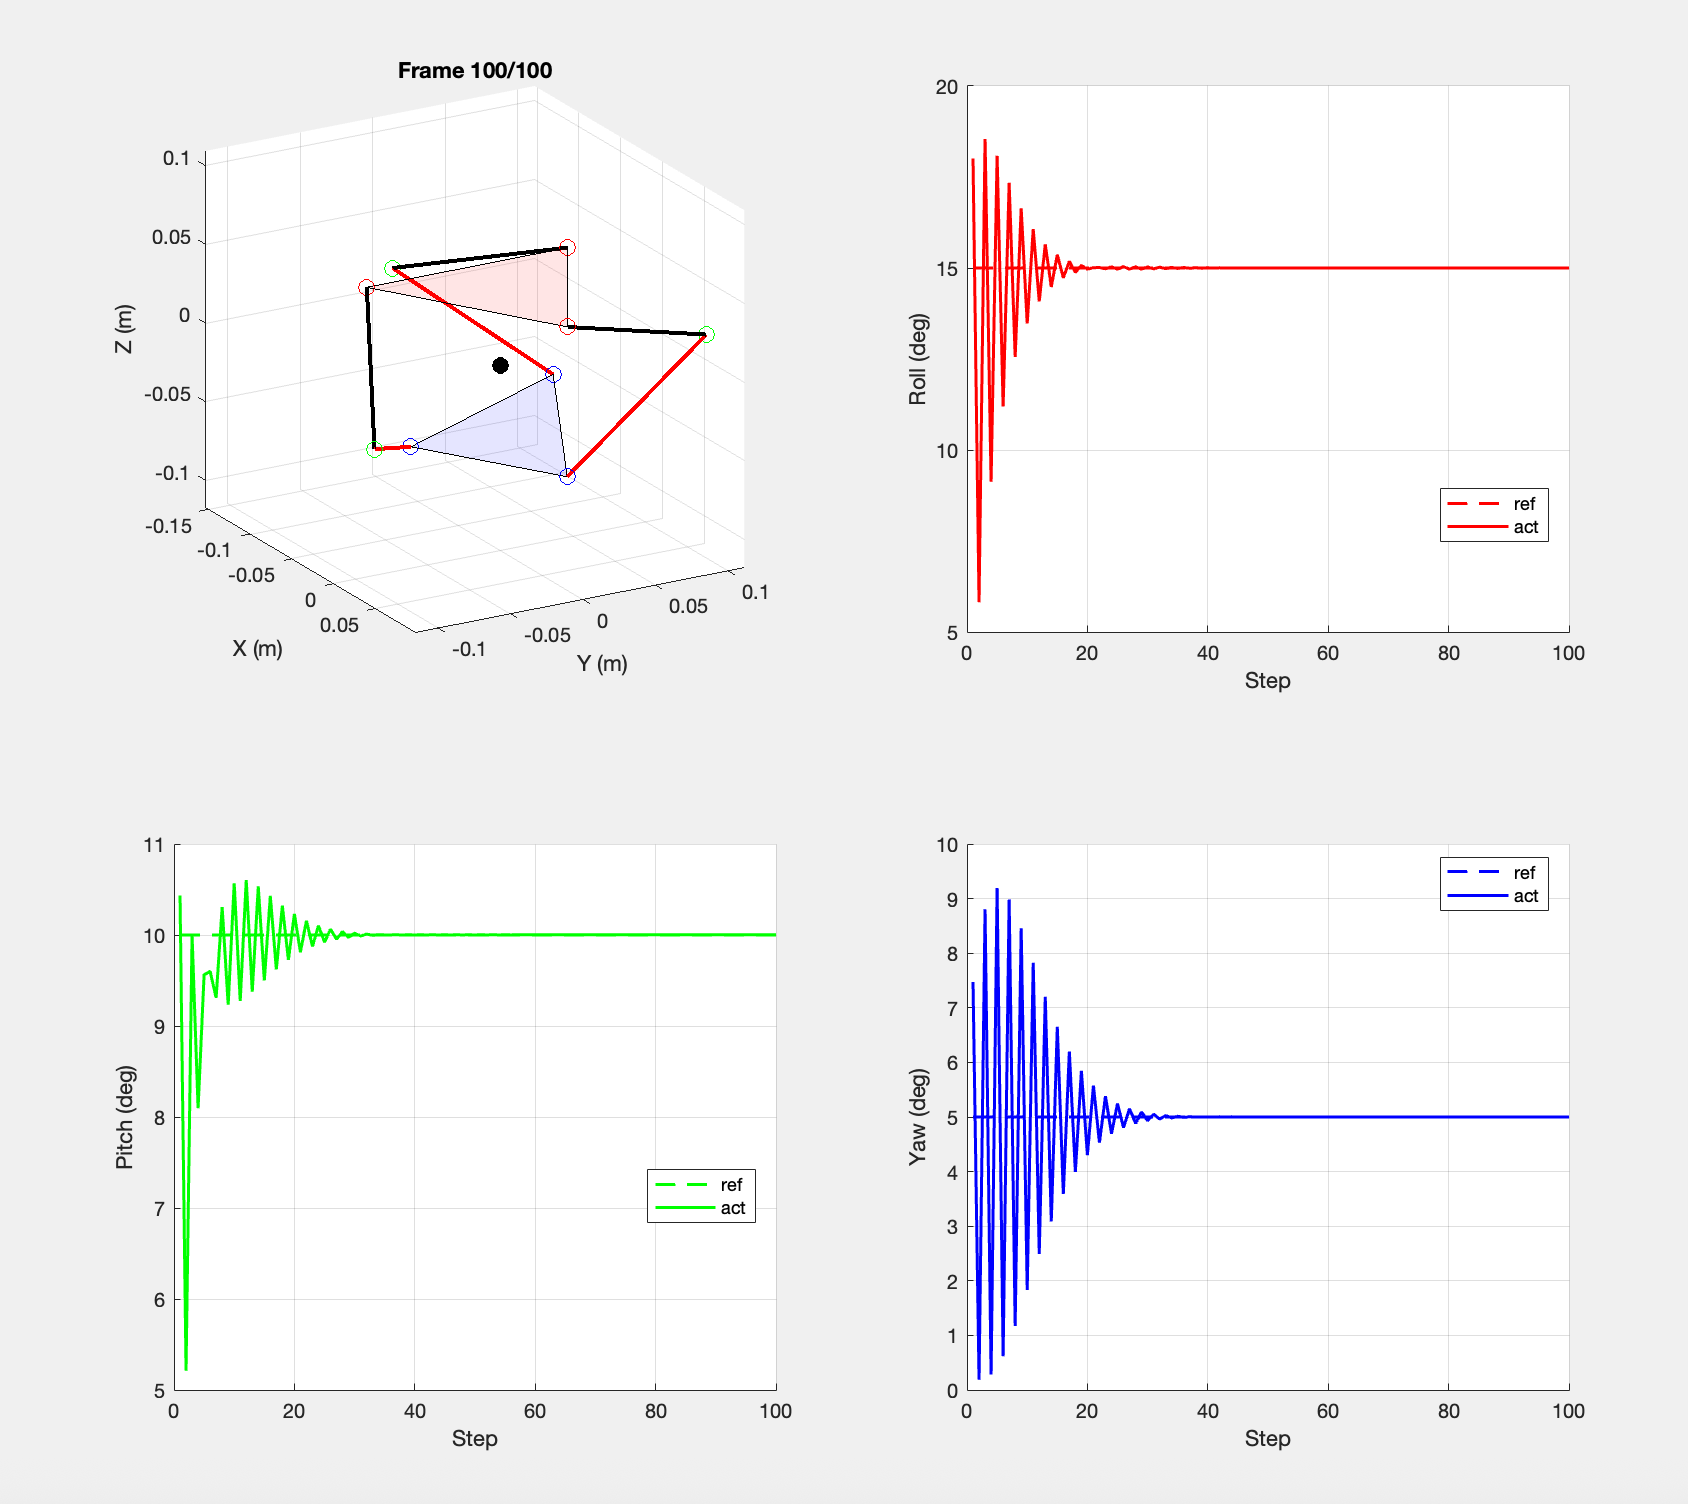
\includegraphics[width=\linewidth]{critical_response.png}
\caption{Critically damped tuning $(K_p,K_d,K_i)=(50,2,5)$.}
\label{fig:pid-crit}
\end{subfigure}
\caption{Platform orientation tracking under the two PID baselines for a step reference $[15^{\circ},10^{\circ},5^{\circ}]^{\!T}$ in (roll, pitch, yaw). The low-stiffness tuning (a) yields oscillatory settling, emulating a soft, compliant interaction. The high-stiffness tuning (b) produces fast, non-oscillatory convergence. The two regimes bracket the spectrum of stiffness that the AAN controller of Section~\ref{sec:aan} interpolates online.}
\label{fig:pid-baseline}
\end{figure}

\section{Assist-As-Needed Control Strategy}
\label{sec:aan}

\subsection{Dual-Mode Rehabilitation}

The proposed device supports two complementary rehabilitation modes that share the same low-level controller:
\begin{enumerate}
\item \textbf{Passive (CPM) mode}: the robot drives the foot plate along a predefined trajectory regardless of patient effort, mimicking the continuous passive motion commonly prescribed in early-stage rehabilitation.
\item \textbf{Active (AAN) mode}: the robot intervenes only when the patient cannot keep up with the desired trajectory, encouraging voluntary effort and motor learning.
\end{enumerate}
The two modes differ in how the reference trajectory and the assistance gain are computed. Mode arbitration is performed by a finite-state supervisor that uses gait-mat events and clinician-prescribed protocols. Figure~\ref{fig:aan-architecture} summarizes the overall control architecture as adopted from a representative AAN exoskeleton design~\cite{jackson2019heuristic,perez2024modeling}: gait-phase extraction and inter-limb asymmetry detection feed an AAN supervisor that adapts the assistance torque, while a low-level force-tracking inner loop closes the actuator current.

\begin{figure}[!t]
\centering
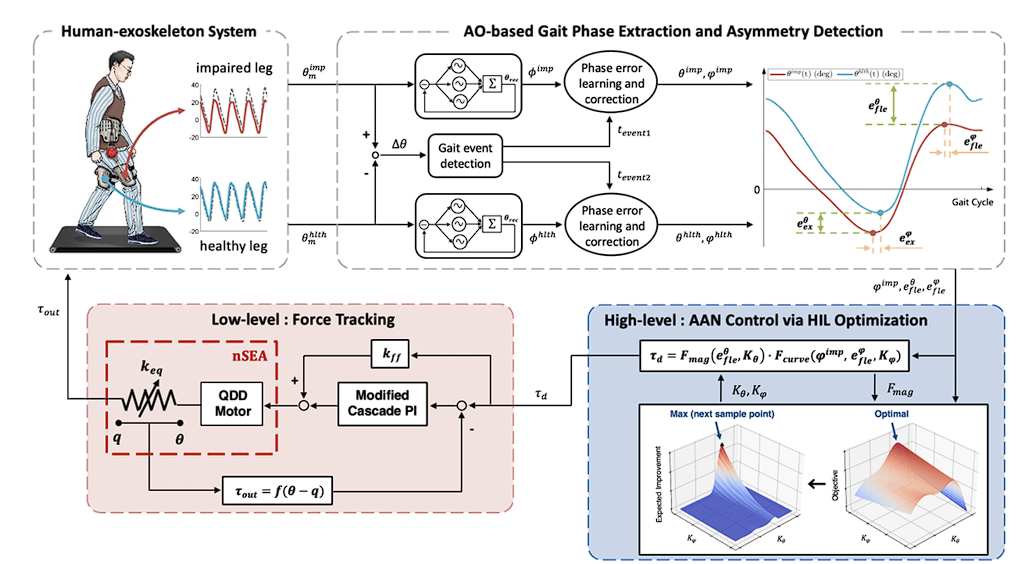
\includegraphics[width=\linewidth]{aan_architecture.png}
\caption{Conceptual control architecture for the proposed device, adapted to the 3-RRR SPM. \emph{Top:} a high-level supervisor extracts per-stride gait phase from sensor data and detects inter-limb asymmetry between an impaired and a healthy reference cycle. \emph{Bottom-right:} the AAN block schedules the assistance torque $\tau_d$ as a function of the asymmetry signals; \emph{bottom-left:} a low-level force-tracking loop drives the actuator current to deliver $\tau_d$ and reports the measured interaction torque back to the supervisor. The same architecture is realized on the proposed device by replacing the series-elastic actuator with the XM430-W350-R current-mode actuator described in Section~\ref{sec:hardware}.}
\label{fig:aan-architecture}
\end{figure}

\subsection{Patient-Torque Estimation from Motor Current}

A central practical question is how to estimate the patient's voluntary contribution without a distal force/torque sensor. The XM430-W350-R provides a calibrated motor current measurement that, combined with the manufacturer's torque constant $K_{t,i}$, yields the actuator torque
\begin{equation}
\hat{\tau}_{\mathrm{act},i}=K_{t,i}\,I_{m,i}.
\end{equation}
Subtracting the model-predicted dynamic torque from \eqref{eq:dynamics} yields an estimate of the patient-applied torque:
\begin{equation}
\tau_{\mathrm{ext},i}\;\approx\;K_{t,i}\,I_{m,i}\;-\;\hat{\tau}_{\mathrm{model},i}(\boldsymbol{q},\dot{\boldsymbol{q}},\ddot{\boldsymbol{q}}_{\mathrm{ref}}),
\label{eq:tau_ext}
\end{equation}
where $\hat{\tau}_{\mathrm{model},i}$ includes the inertial and Coriolis terms (gravity is negligible for an SPM rotating about a fixed center). This ``sensorless'' torque-estimation strategy is consistent with prior practice in ankle-exoskeleton control~\cite{zhang2015torque,jackson2019heuristic} and removes the need for a distal six-axis load cell, an important consideration for distal-mass-sensitive wearable devices.

\subsection{AAN Assistance Law}

For each active joint, the assistance torque is computed as
\begin{equation}
\tau_{\mathrm{assist},i}=k_{\mathrm{aan}}(t,e_i)\,\big[\tau_{\mathrm{ref},i}-\tau_{\mathrm{ext},i}\big]_+,
\label{eq:tau_assist}
\end{equation}
where $\tau_{\mathrm{ref},i}$ is the model-based torque required to follow the reference trajectory, $[\,\cdot\,]_+$ denotes the positive part, and $k_{\mathrm{aan}}(t,e_i)\in[0,1]$ is an adaptive gain that grows with tracking error $e_i=q_{i,\mathrm{ref}}-q_i$ and decays with successful tracking. Concretely, we use
\begin{equation}
k_{\mathrm{aan}}(t,e_i)=\mathrm{sat}_{[0,1]}\!\left(k_0+k_e\,|e_i|-k_s\right),
\end{equation}
where $k_0$ is a small baseline, $k_e>0$ is an error-dependent rise rate, and $k_s>0$ is a forgetting term that decays the gain when tracking is consistent. This produces the desired AAN behavior: the robot does not assist as long as the user can follow the trajectory, and ramps up assistance only when needed, in line with the principles articulated by Reinkensmeyer and colleagues~\cite{cai2006implications,marchal2009review}.

\subsection{Safety Supervision}

A safety supervisor enforces:
\begin{itemize}
\item per-joint angle and velocity limits derived from the optimized workspace and clinician-prescribed range of motion;
\item per-motor current limits below the XM430-W350-R stall current;
\item soft-start and soft-stop ramps at the start and end of every trajectory;
\item online monitoring of $\kappa(\mathbf{J}_r)$ via \eqref{eq:jacobian}, which scales velocity commands down as the platform approaches singular configurations;
\item dropout pause when IMU or gait-mat data are missing or stale; and
\item a hardware emergency-stop input that opens the actuator power line.
\end{itemize}

\section{Embedded System and Sensor Architecture}
\label{sec:hardware}

\subsection{Master Controller and Actuator Bus}

The on-device computer is a Teensy~4.1, an ARM Cortex-M7 microcontroller running at 600\,MHz that provides deterministic, low-latency execution suitable for medical-grade closed-loop control. The Teensy~4.1 hosts a 1~kHz control loop that performs (i) IMU acquisition, (ii) numerical IK, (iii) AAN torque computation, (iv) safety checks, and (v) actuator command transmission, with sufficient headroom for online estimation routines. A 1~kHz loop rate is consistent with prior practice in ankle-exoskeleton control where stable force-feedback loops are required~\cite{zhang2015torque,jackson2019heuristic}.

The actuators communicate with the master over a single RS-485 daisy-chain bus, which simplifies wiring and reduces the cable mass on the limb. The XM430-W350-R operates in the manufacturer's current-based position-control mode, in which the user commands a position setpoint and a current saturation, while the actuator returns position, velocity, and current measurements~\cite{robotisxm430}. The position encoding is
\begin{equation}
\mathrm{tick}=2048+\frac{\theta_{\deg}}{0.087912},
\end{equation}
giving a resolution of approximately $0.088^{\circ}$ per tick across the full $0$--$4095$ tick range, sufficient for the angular resolutions required in ankle rehabilitation. Figure~\ref{fig:hardware} shows the prototype electronics stack used for early integration of the master, IMU, and RS-485 bus.

\begin{figure}[!t]
\centering
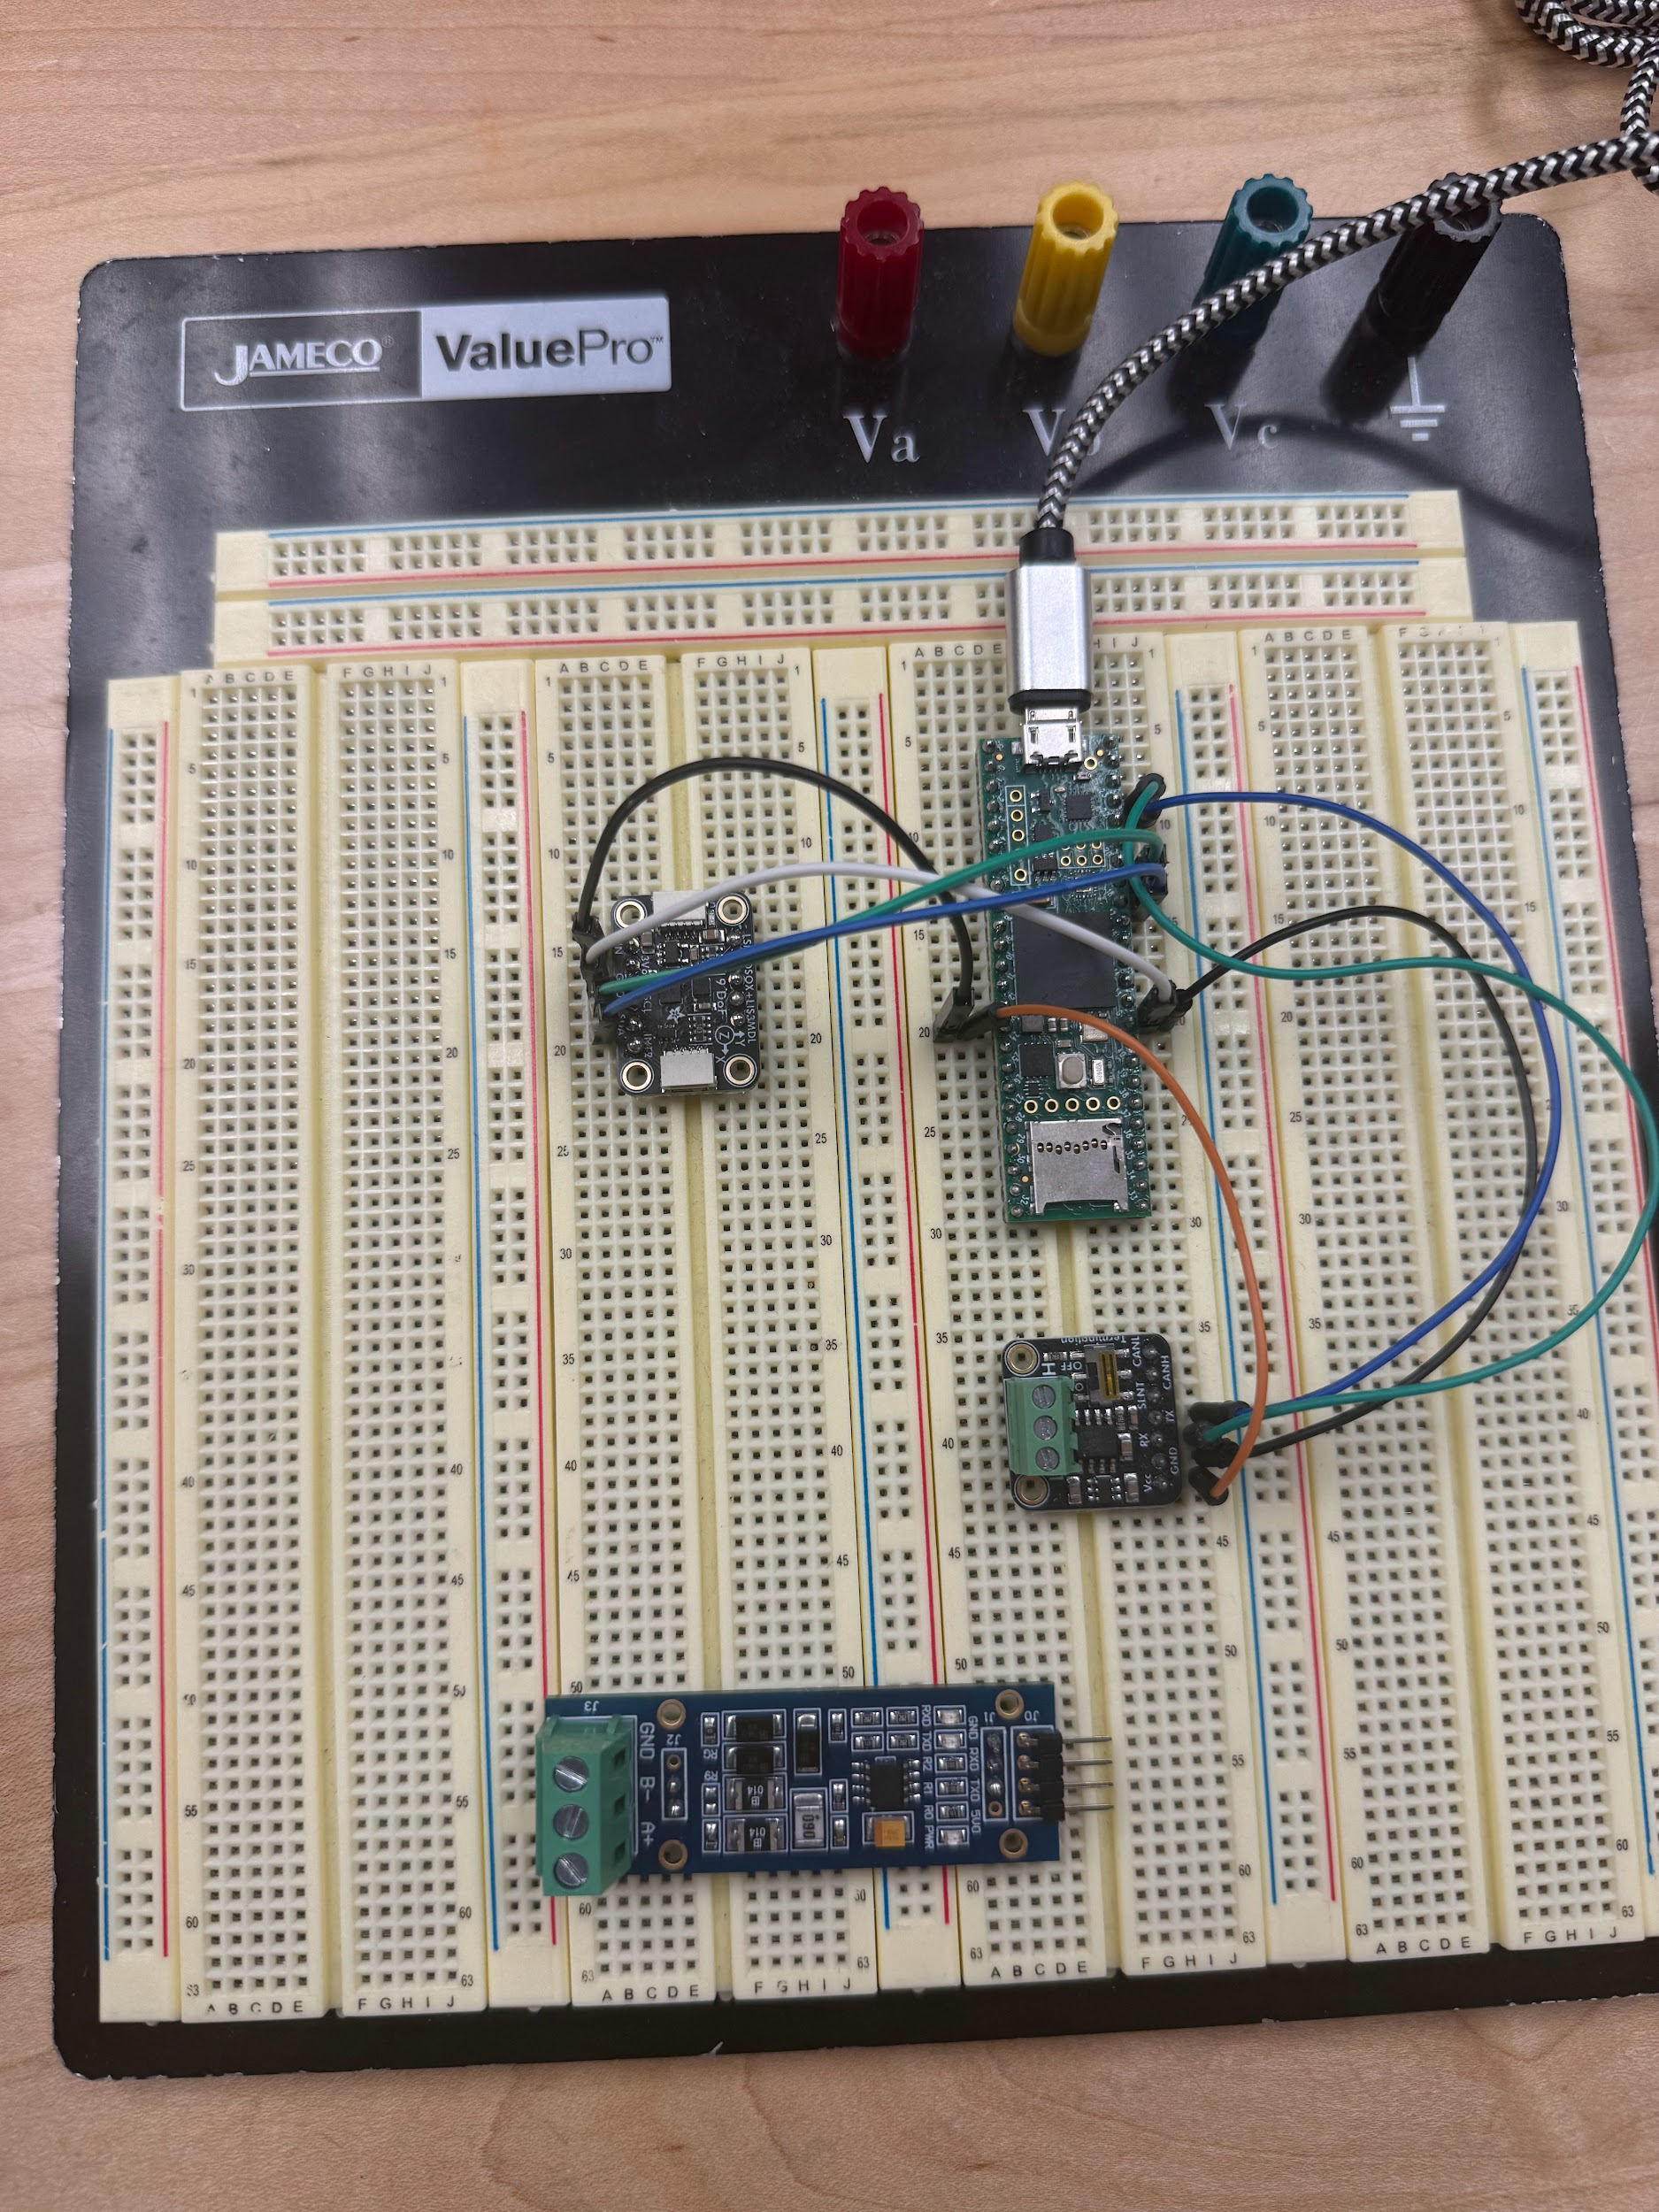
\includegraphics[width=0.78\linewidth]{electronics_breadboard.jpg}
\caption{Prototype electronics stack on a breadboard for early integration. A Teensy~4.1 master controller (center) communicates with an IMU breakout (left) for shank/foot orientation and a TTL-to-RS-485 transceiver (bottom) that bridges the master to the daisy-chained Dynamixel XM430-W350-R actuator bus described in Section~\ref{sec:hardware}. The actuator current measurement returned over the same bus feeds the sensorless torque estimator of \eqref{eq:tau_ext}.}
\label{fig:hardware}
\end{figure}

\subsection{Sensor Suite}

Three classes of sensors are integrated:
\begin{itemize}
\item \textbf{Motor encoders.} Each XM430-W350-R reports relative joint angle, velocity, and current at the 1~kHz loop rate. The current measurement is used directly in the AAN torque estimator \eqref{eq:tau_ext}.
\item \textbf{Inertial measurement units.} Two IMUs are mounted on the lower limb. One is fixed to the patient's tibia (shank), and the other to the dorsum of the foot or directly to the moving platform. While the encoders measure relative joint angles, the dual-IMU arrangement provides absolute orientation referenced to gravity, which is essential both for the AAN reference and for cross-validating the IK output~\cite{yue2018wearable}.
\item \textbf{Gait mat and external pose tracker.} A laboratory gait mat measures stance time, plantar pressure distribution, and the CoP trajectory, mirroring the instrumented-shoe pipeline of Prado \emph{et al.}~\cite{prado2020fog} and Paydarfar \emph{et al.}~\cite{paydarfar2020rnn}. An HTC Vive tracker is used as a high-precision external reference for foot-plate orientation during calibration of the kinematic parameters and for periodic re-validation.
\end{itemize}

\subsection{Wearable Form Factor}

The 3D-printed prototype provides a functional but coarse human interface. Planned hardware iteration adds a foam insole and soft padding inside the foot brace and around the base ring strap to reduce localized skin pressure during extended training sessions. A low-profile cable management strategy following~\cite{yandell2019profile} routes the actuator wiring along the medial side of the limb to avoid interference with footwear or orthoses.

\section{Open-Source Implementation and Simulation Pipeline}
\label{sec:opensource}

To support reproducibility and to lower the barrier to extending this work, the entire software stack of the device is publicly released under the MIT license at \url{https://github.com/YufeiZhang0601/wearable-3rrr-ankle-rehab}. The release goes beyond a CAD dump: it provides an executable simulation pipeline, a parallel-IK solver, ROS\,2 launch and node code, and a dependency-free closed-loop demo, so that a new contributor can clone the repository and reproduce the kinematic and visualization results without owning the hardware.

\subsection{Repository Layout}

The repository is organized as a single ROS\,2 \texttt{ament\_python} package named \texttt{rh1}, with the layout summarized in Table~\ref{tab:repo}. The Python module exposes the kinematic core, the launch and config trees provide ROS\,2-friendly entry points, the URDF and meshes describe the device, and a \texttt{scripts/} directory ships standalone CLI tools that do not require a ROS environment.

\begin{table}[!t]
\centering
\caption{Open-source repository layout (selected entries).}
\label{tab:repo}
\begin{tabular}{p{0.31\linewidth} p{0.61\linewidth}}
\toprule
\textbf{Path} & \textbf{Contents}\\
\midrule
\texttt{rh1/parallel\_ik.py}            & numerical parallel-IK solver\\
\texttt{rh1/parallel\_ik\_pose\_demo.py}  & ROS\,2 node: command (roll, pitch, yaw)\\
\texttt{rh1/ankle\_rehab\_control.py}     & shared trajectory + safety utilities\\
\texttt{urdf/rh1.urdf}                   & full URDF exported from SolidWorks\\
\texttt{urdf/rh1\_sim.urdf.xacro}        & lightweight RViz/Gazebo model\\
\texttt{meshes/\{visual,collision\}/}    & 22 STL meshes referenced by the URDF\\
\texttt{launch/}                         & display, ankle-rehab demo, IK pose demo, Gazebo launch files\\
\texttt{scripts/ankle\_rehab\_closed\_loop\_demo.py} & dependency-free closed-loop tracking demo with CSV log\\
\texttt{scripts/extract\_step\_kinematics.py}        & mines kinematic candidates from a STEP assembly\\
\texttt{scripts/auto\_generate\_parallel\_ik\_params.py} & bootstraps IK parameters from CAD extraction\\
\texttt{params/}                         & kinematic and parallel-IK parameter templates\\
\texttt{report/}                         & LaTeX sources of this report\\
\texttt{media/closed\_loop\_demo.mp4}    & screen capture of the closed-loop demo\\
\bottomrule
\end{tabular}
\end{table}

\subsection{Parallel Inverse-Kinematics Solver}

The Python module \texttt{rh1/parallel\_ik.py} implements the numerical IK formulation of Section~\ref{sec:kinematics}. For each requested foot-plate pose, the solver evaluates the leg constraint of \eqref{eq:leg-constraint} on a discretized motor-angle bracket, switches to bisection inside the active bracket, and selects the root closest to the previous time step to enforce branch continuity. The solver is intentionally dependency-free (only the Python standard library), so it runs both inside ROS\,2 and on a host laptop without ROS.

A one-shot CLI wrapper \texttt{scripts/parallel\_ik\_demo.py} exposes the solver to a terminal user:
\begin{verbatim}
python scripts/parallel_ik_demo.py \
  --roll-deg 5 --pitch-deg 10 --yaw-deg 0
\end{verbatim}
prints the three motor angles in degrees, in radians, and in Dynamixel ticks (using the encoding of \eqref{eq:active-angle} and the tick formula in Section~\ref{sec:hardware}), enabling rapid trajectory pre-checks before the same command is sent to the real bus.

\subsection{ROS\,2 Visualization and Closed-Loop Demo}

The package ships four ROS\,2 launch files: \texttt{display\_robot.launch.py} (static URDF in RViz), \texttt{ankle\_rehab\_demo.launch.py} (a scripted ankle rehab trajectory with a \texttt{JointState} player), \texttt{parallel\_ik\_pose\_demo.launch.py} (interactive (roll, pitch, yaw) command using the parallel-IK solver), and \texttt{gazebo.launch.py} (Gazebo bring-up). All four reuse the same URDF / Xacro and the same Python kinematic core, so behaviour is consistent across pure-Python, RViz, and Gazebo entry points.

In parallel, \texttt{scripts/ankle\_rehab\_closed\_loop\_demo.py} provides a dependency-free closed-loop demo. It parses \texttt{urdf/rh1.urdf}, treats \texttt{joint1}, \texttt{joint4}, and \texttt{joint6} as the three Dynamixel XM430-W350-R virtual actuators, runs a simple position-tracking controller on a slow, low-amplitude rehab trajectory (12$^{\circ}$ dorsiflexion / plantarflexion amplitude, 6$^{\circ}$ inversion / eversion amplitude, 0.05~Hz, 3-s soft start), enforces a conservative 1.2~Nm patient-side torque cap and 0.8~rad/s velocity cap, and writes per-cycle feedback (commanded vs.\ measured joint angles, residual tracking error, and Dynamixel goal ticks) to \texttt{demo\_output/ankle\_rehab\_closed\_loop.csv}. The full screen capture of the demo is included in the repository as \texttt{media/closed\_loop\_demo.mp4} (\textasciitilde 25\,MB).

\subsection{Gazebo Verification of the URDF}

Beyond visualization, the URDF was loaded into Gazebo to verify that the closed-chain joint axes and inertial parameters behave physically when an external load is applied. Figure~\ref{fig:gazebo-ft} shows the \emph{Apply Force and Torque} dialog being used to inject a $\sim 100$~Nm pure torque on \texttt{Link1} (purple torque arrow visible in the viewport, with the smaller red wireframe widget marking the application point at the link's center of mass). Sweeping the application link, force/torque magnitudes, and Cartesian application points across a representative grid did not reveal abnormal pose drifts, NaN inertia errors, or mesh-collision interpenetration. This Gazebo-based smoke test gates each URDF change before it lands in the \texttt{main} branch.

\begin{figure}[!t]
\centering
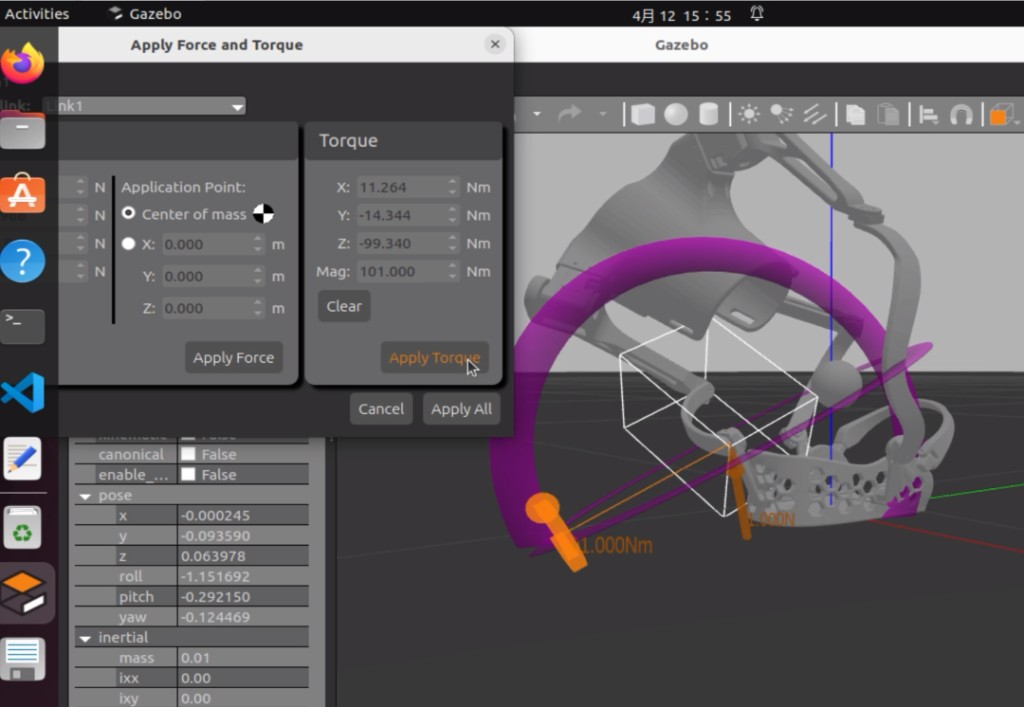
\includegraphics[width=\linewidth]{gazebo_force_torque.png}
\caption{Gazebo verification of the URDF / Xacro model. The \emph{Apply Force and Torque} dialog is being used to inject a 101~Nm pure torque (with components $T_x{=}11.3$, $T_y{=}{-}14.3$, $T_z{=}{-}99.3$~Nm) on \texttt{Link1} at the link's center of mass; the purple torque arrow in the viewport is Gazebo's visualization of the applied torque, and the small wireframe widget marks the application point. The lower-left property panel shows the link pose (roll, pitch, yaw of $-1.152$, $-0.292$, $-0.124$~rad) and the inertial entries that the URDF defines, both of which are checked against the SolidWorks export. Tests of this kind are scripted into a Gazebo smoke test that gates each URDF change in the open-source repository (Section~\ref{sec:opensource}).}
\label{fig:gazebo-ft}
\end{figure}

\subsection{Reproducibility and Extension}

A new user reproduces the simulation results in three steps: (i) clone the repository; (ii) run \texttt{python scripts/ankle\_rehab\_closed\_loop\_demo.py} for the standalone closed-loop demo; (iii) build the package in a ROS\,2 (Humble or later) workspace and \texttt{ros2 launch rh1 parallel\_ik\_pose\_demo.launch.py} for the interactive pose demo. Parameter overrides for the link geometry and motor zero offsets live entirely in \texttt{params/parallel\_ik\_params.\{template,example,autogenerated\}.json}, so a researcher swapping in different physical hardware does not need to modify any Python code.

\section{Experimental Methodology}
\label{sec:experiments}

This section defines the experimental protocol used to evaluate the device. Three categories of active-rehabilitation experiments and one passive transfer-effect experiment share a common set of quantitative metrics and a common analysis pipeline. The reference clinical practice that the device is designed to standardize and complement is illustrated in Fig.~\ref{fig:manual-therapy}: a clinician's manual mobilization of the talocrural, subtalar, and distal tibiofibular joints in both anterior--posterior and posterior--anterior directions. By replicating these mobilization patterns under quantitative control, the proposed device aims to reduce inter-clinician variability and produce dose-controlled therapy.

\begin{figure}[!t]
\centering
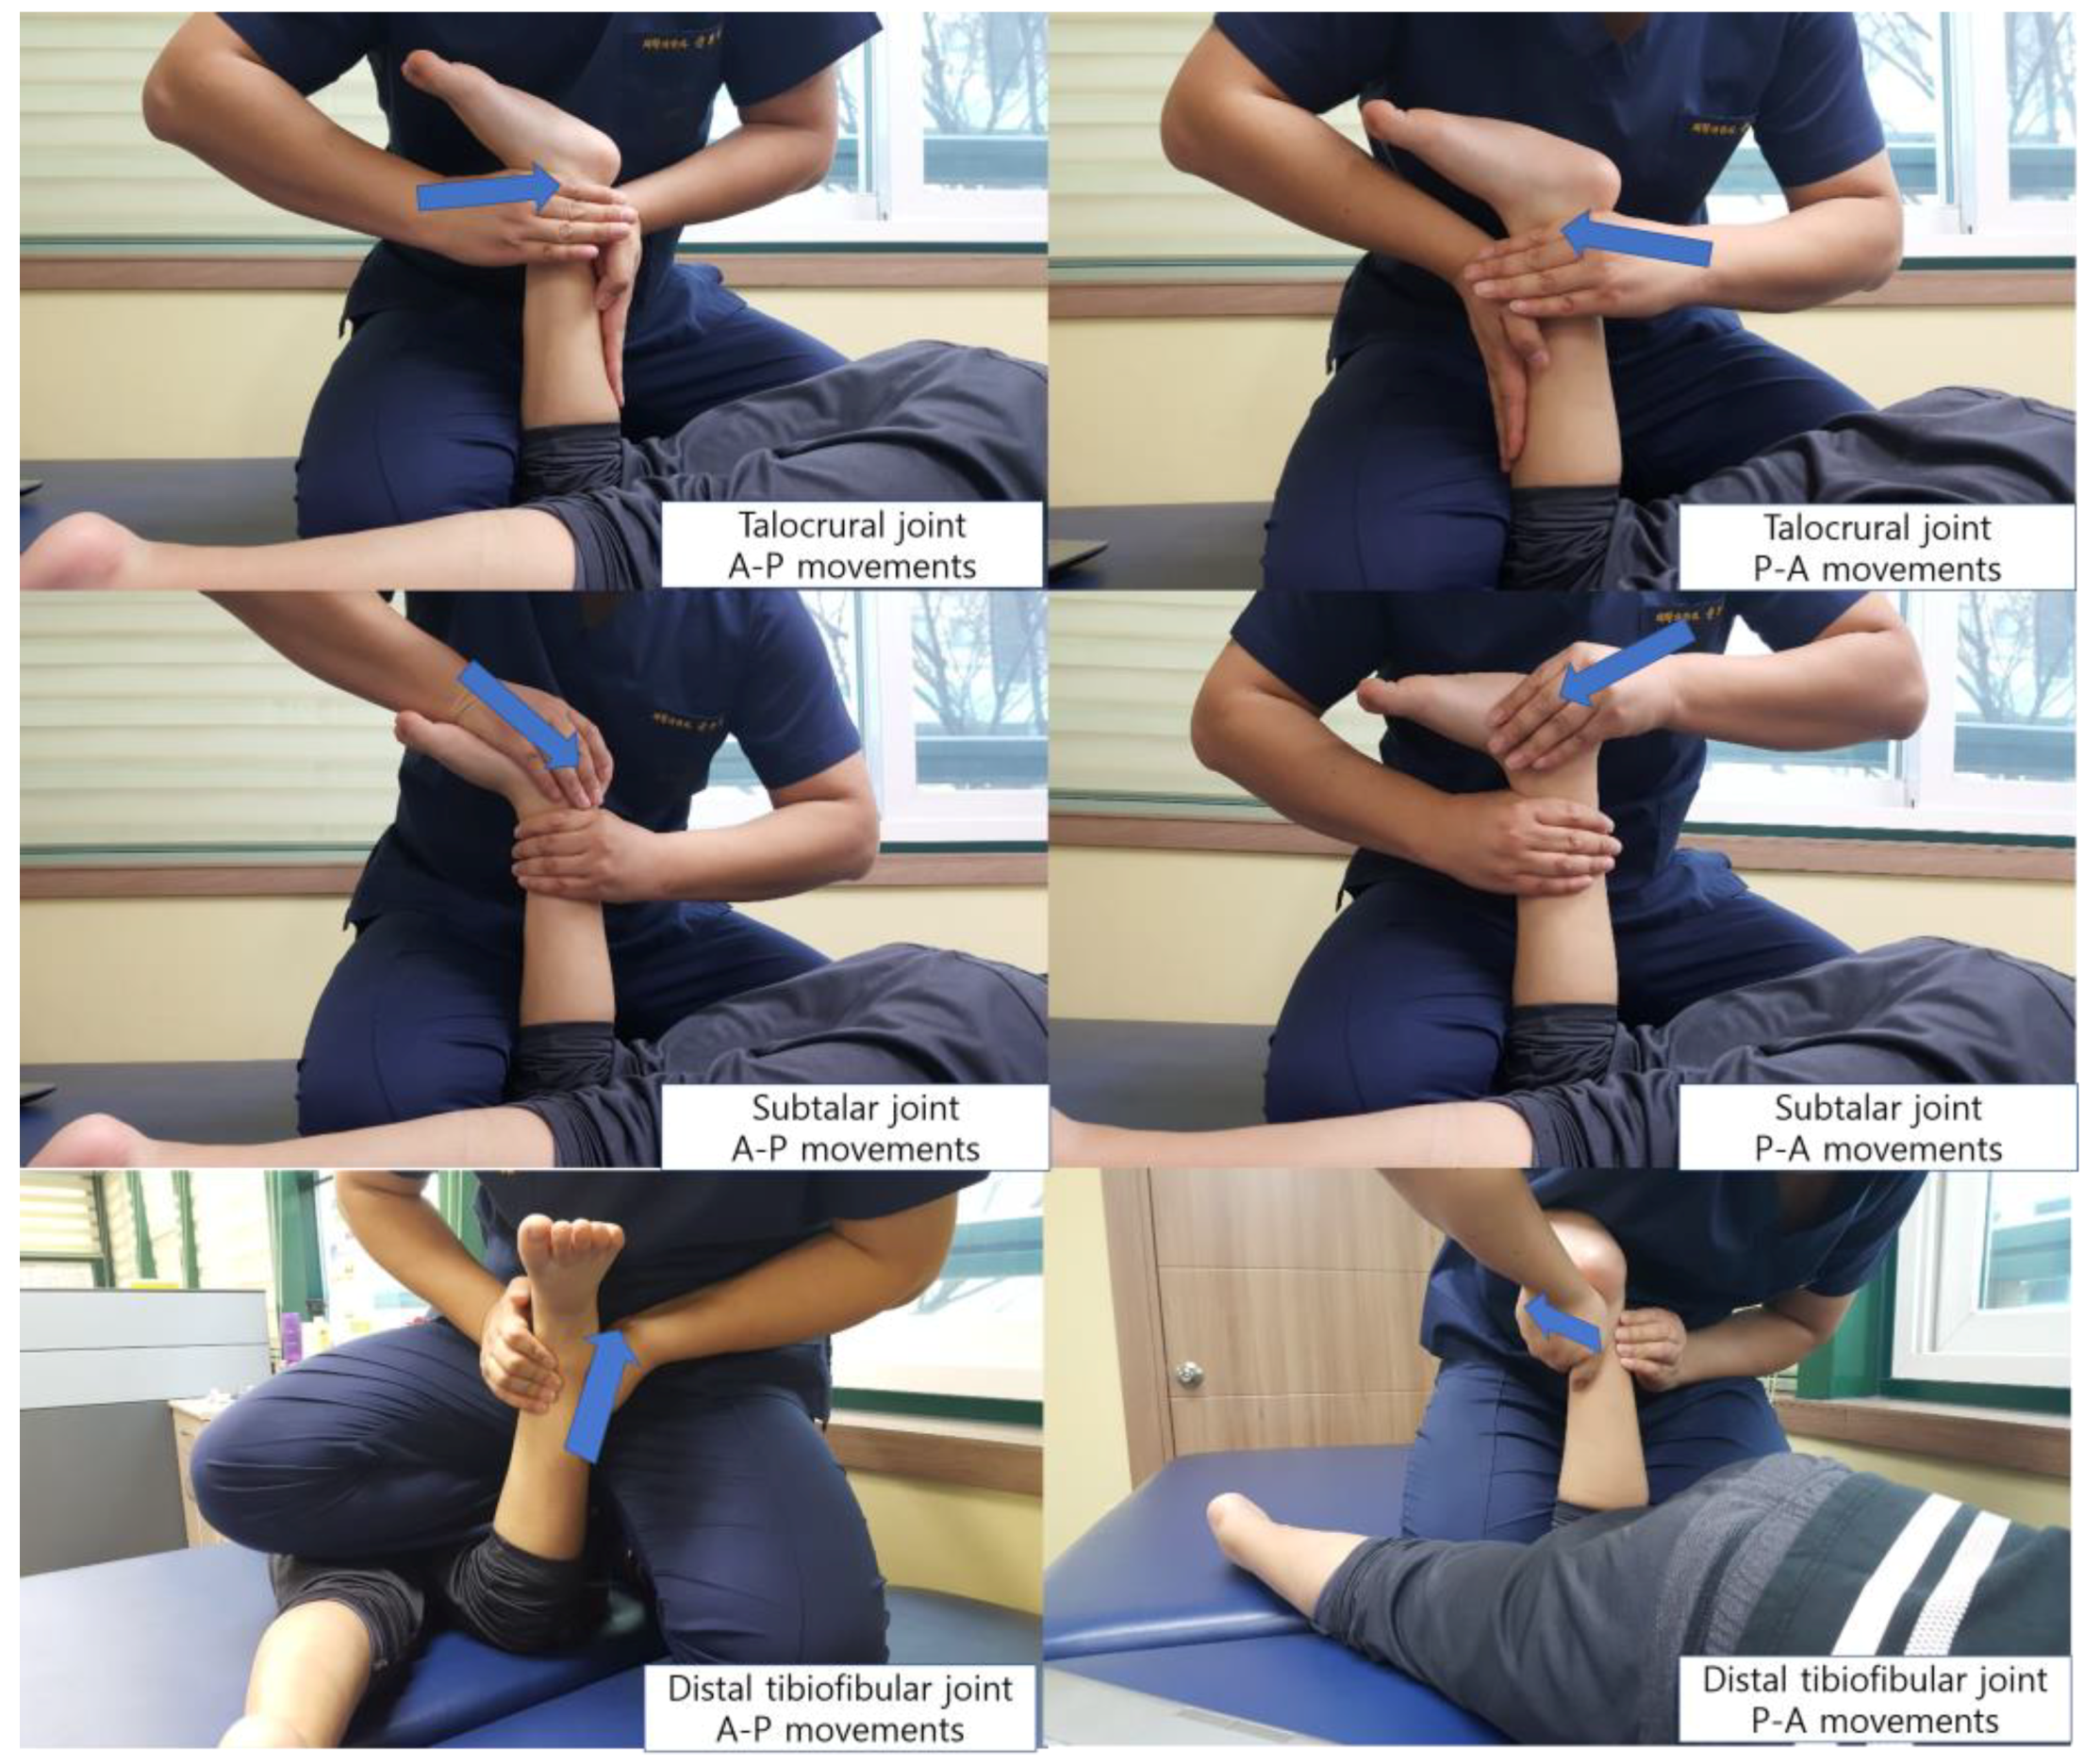
\includegraphics[width=0.85\linewidth]{manual_therapy.png}
\caption{Clinical reference: manual ankle mobilization of the talocrural, subtalar, and distal tibiofibular joints in both A--P and P--A directions, as performed by a physical therapist. Therapist-driven manual therapy of this type is the dominant standard of care, but it is highly dependent on clinician experience and provides only qualitative dosing. The proposed robotic device targets the same biomechanical motions while providing quantitative trajectory tracking, interaction-torque estimation, and outcome metrics. Image adapted from clinical rehabilitation literature.}
\label{fig:manual-therapy}
\end{figure}

\subsection{Quantitative Metrics}

The primary metrics, drawn from the rehabilitation-robotics literature, are:
\begin{itemize}
\item \textbf{Limb Symmetry Index (LSI)}, the ratio of an outcome variable measured on the affected versus the unaffected limb, computed for peak ankle range of motion (ROM), peak plantar pressure, and stance time. LSI is the ``north-star'' clinical metric: scores in the 90--110\% band are conventionally regarded as restored symmetry~\cite{hidayah2020calex}.
\item \textbf{Jerk}, the time derivative of acceleration, computed from the foot-plate IMU and used as a smoothness indicator. Smoother trajectories correlate with motor-skill consolidation~\cite{marchal2009review}.
\item \textbf{Interaction torque} $\tau_{\mathrm{int}}$ between device and patient, estimated via the AAN torque estimator \eqref{eq:tau_ext} and reported in Newton-meters per gait cycle.
\item \textbf{Center of Pressure (CoP)} from the gait mat, reported for both static stance and dynamic gait cycles.
\item \textbf{Human-contribution ratio} $\eta_h=\tau_{\mathrm{ext}}/(\tau_{\mathrm{ext}}+\tau_{\mathrm{assist}})$, indicating the fraction of total joint torque produced by the patient under AAN.
\end{itemize}

\subsection{Subject Cohort and Controlled-Deficit Induction}

Initial subjects are three healthy team members. To create a controlled and ethically tractable functional deficit, we induce a \emph{simulated foot-drop} condition by either (a) attaching a small calibrated weight near the toe, increasing the swing-phase plantarflexion moment and forcing the participant to compensate, or (b) commanding a downward (plantarflexion) bias torque on the device's distal limb, which the participant must overcome to achieve dorsiflexion. Both methods are reversible, do not require an IRB-regulated patient population, and produce a measurable LSI deviation that mirrors clinical foot-drop without exposing impaired participants. A baseline (no-deficit, no-device) condition and a deficit-only (no-device) condition are also recorded for each subject to establish within-subject baselines.

\subsection{Experiment 1: Simulated-Impairment Recovery}

\textbf{Hypothesis.} AAN training corrects the abnormal gait pattern induced by the simulated deficit, with measurable improvement in LSI and reduction of compensatory motions (e.g., hip hiking).

\textbf{Protocol.} Each subject completes four conditions: baseline walking; deficit-only walking; deficit walking with the device in transparent mode; and deficit walking with the device in AAN mode. Each condition consists of a 5-minute walking trial on the gait mat at a self-selected speed. The peak ankle ROM, plantar-pressure peak, stance time, hip joint excursion, and IMU-derived foot-clearance metric are extracted from the central 90~s of each trial.

\textbf{Outcome.} A successful outcome is an LSI improvement from $\sim 80\%$ in the deficit-only condition toward $\sim 95\%$ in the AAN condition, accompanied by a measurable reduction in hip-hiking range, in line with the kind of changes reported by Hidayah \emph{et al.}~\cite{hidayah2020calex} for stroke participants under cable-driven exoskeleton training.

\subsection{Experiment 2: Transparency Evaluation}

\textbf{Hypothesis.} Under near-zero-impedance control, the device does not appreciably alter natural ankle kinematics or impose significant interaction torques on the user.

\textbf{Protocol.} The controller is placed in a transparency mode that suppresses all assistance and applies only a low-gain damping term sufficient to suppress motor friction. Each subject walks 5~minutes barefoot on the gait mat (Condition~A) and 5~minutes wearing the device in transparent mode (Condition~B). The IMU-derived ankle angle trajectory and the gait-mat-derived CoP trajectory are compared between conditions using stride-normalized signals.

\textbf{Outcome.} The system is considered approximately transparent if the inter-condition similarity satisfies $R^2 > 0.95$ on the stride-normalized ankle angle and $|\tau_{\mathrm{int}}| \to 0$ throughout the gait cycle, in line with the transparency criteria reported in~\cite{galle2013adaptation,jackson2019heuristic}.

\subsection{Experiment 3: Active Participation under AAN}

\textbf{Hypothesis.} Under AAN control, the human-contribution ratio $\eta_h$ increases across training sessions while the jerk-based smoothness index remains within a stability band, indicating that AAN promotes voluntary effort without destabilizing motion.

\textbf{Protocol.} Each subject completes five 10-minute AAN training sessions on consecutive days. Within each session, $\eta_h$ and the per-stride jerk are computed and reported as session-mean values with 95\% confidence intervals. A linear mixed-effects model is used to assess the across-session trend, with subject as a random effect.

\textbf{Outcome.} A rising $\eta_h$ and a stable jerk profile would indicate that the AAN gain is correctly modulating assistance: enough to permit successful trajectory completion early in training, but progressively less as the user re-acquires the skill, consistent with the motor-learning theory underlying AAN~\cite{cai2006implications,marchal2009review}.

\subsection{Experiment 4: Passive Transfer Effect}

\textbf{Hypothesis.} A short bout of passive (CPM) training on the device, with enhanced dorsiflexion amplitude, produces a short-term carryover in overground gait, manifested as an increase in step length and a forward shift of the CoP.

\textbf{Protocol.} Each subject performs a baseline overground walking trial; then 10~minutes of seated, passive CPM training on the device with prescribed dorsiflexion amplitude; and finally a post-training overground walking trial. Step length and CoP are extracted from the gait mat in both walking trials. Within-subject pre/post differences are tested using paired $t$-tests with Bonferroni correction.

\textbf{Outcome.} A consistent post-training increase in step length and forward CoP shift would indicate that the device modulates the patient's neural control strategy beyond the immediate biomechanical effect of wearing it, mirroring the transfer-effect framework used in~\cite{galle2013adaptation,gordon2007learning}.

\subsection{Sensing Pipeline and Data Synchronization}

All sensor streams are time-stamped on the Teensy~4.1 with a common monotonic clock. IMU data are sampled at 200~Hz, motor data at the controller's 1~kHz loop rate (down-sampled for logging), and the gait-mat events are received over Ethernet at the mat's native frame rate. Data are streamed to a host laptop for off-line analysis. Per-stride segmentation uses heel-strike events from the foot IMU, validated against gait-mat contacts. Activity classification baselines following~\cite{paydarfar2020rnn} are reserved for future work.

\subsection{Statistical Analysis}

Group-level statistics are reported as mean $\pm$ standard deviation, with 95\% confidence intervals computed by bootstrap resampling ($n=10000$). Within-subject paired comparisons use paired $t$-tests when normality is supported by a Shapiro-Wilk test; otherwise, Wilcoxon signed-rank tests are used. Multiple-comparison corrections are applied at the experiment level using the Bonferroni-Holm procedure. Across-session trends are analyzed using linear mixed-effects models with subject as a random effect.

\section{Implementation Status}
\label{sec:results}

Table~\ref{tab:goals} summarizes the status of the research goals proposed in this report. Five of the six goals are complete and reproducible from the open-source repository introduced in Section~\ref{sec:opensource}; the remaining goal---hardware integration with a real Dynamixel bus and the human-subject experiments described in Section~\ref{sec:experiments}---is in progress.

\begin{table}[!t]
\centering
\caption{Status of proposed goals.}
\label{tab:goals}
\begin{tabular}{p{0.40\linewidth} p{0.20\linewidth} p{0.30\linewidth}}
\toprule
\textbf{Goal} & \textbf{Status} & \textbf{Outcome}\\
\midrule
Wearable 3-RRR mechanism with structurally favourable link ratio & Completed & $l_2/l_1\approx 1.15$, isotropy +20\%\\
Closed-form and numerical IK & Completed & Sec.~\ref{sec:kinematics}\\
Joint-to-actuator mapping ($\theta_i \to$ XM430) & Completed & Sec.~\ref{sec:hardware}\\
Open-source ROS\,2 / Gazebo pipeline & Completed & Sec.~\ref{sec:opensource}, MIT-licensed release\\
AAN control formulation & Proposed & Eq.~\eqref{eq:tau_ext}--\eqref{eq:tau_assist}\\
Embedded system architecture & Completed & Teensy~4.1 + RS-485 + dual IMU + gait mat\\
Hardware integration and experiments & In progress & Sec.~\ref{sec:experiments}\\
\bottomrule
\end{tabular}
\end{table}

\section{Conclusion and Future Work}
\label{sec:conclusion}

This report extends our prior 3-RRR ankle rehabilitation robot~\cite{zhang2025rehab} from a CAD-and-prototype snapshot into a reproducible research platform. Three concrete contributions are delivered. First, a wearable 3-RRR SPM embodiment with a structurally favourable link ratio ($l_2/l_1\approx 1.15$) improves the global rotational-Jacobian isotropy by approximately 20\% relative to a naive 1:1 design and pushes parallel singularities toward the workspace boundary. Second, analytical and numerical inverse-kinematic formulations map a clinically meaningful (roll, pitch, yaw) command to the three actuated motor angles in a form suitable for real-time execution on a Teensy~4.1 platform driving Dynamixel XM430-W350-R smart actuators. Third, a complete open-source implementation---ROS\,2 \texttt{ament\_python} package, URDF / Xacro verified in Gazebo, parallel-IK solver, interactive pose demo, and dependency-free closed-loop demo with a recorded video clip---is released under an MIT license at \url{https://github.com/YufeiZhang0601/wearable-3rrr-ankle-rehab}, lowering the barrier for other groups to extend or replicate this work. The proposed AAN control law and the multi-modal sensing protocol provide the framework on which planned hardware-in-the-loop experiments will be built.

Future work falls into three lines. \emph{Modeling}: replace the single-center spherical assumption with a dual-axis non-concentric ankle model that better matches biomechanics, and integrate the Lagrangian dynamic model into a model-based feedforward layer. \emph{Control and software}: instantiate the proposed AAN gain schedule on a real Dynamixel bus inside the open-source pipeline, extend it with fuzzy-logic impedance and gait-phase switching, and incorporate online Jacobian-condition-number monitoring \eqref{eq:jacobian} as an adaptive velocity scaler within the safety supervisor. \emph{Experiments}: complete the planned protocol with healthy subjects, then plan an IRB-approved human-subject study to evaluate alignment, comfort, and therapeutic efficacy in patient populations with foot drop, post-stroke ankle weakness, or chronic ankle instability.

\section*{Acknowledgment}

The author gratefully acknowledges Prof.\ Sunil K.\ Agrawal for his guidance throughout this AMR research project, and the team members and collaborators who contributed to the design, modeling, and evaluation of the proposed system.

\begin{thebibliography}{99}

\bibitem{zhang2025rehab} S.~Zhang, Y.~Zhang, J.~Lyu, and S.~K.~Agrawal, ``From structural design to dynamics modeling: Control-oriented development of a 3-RRR parallel ankle rehabilitation robot,'' \emph{arXiv preprint arXiv:2505.13762}, 2025.

\bibitem{gosselin1989optimum} C.~M.~Gosselin and J.~Angeles, ``The optimum kinematic design of a spherical three-degree-of-freedom parallel manipulator,'' \emph{ASME J.~Mech., Transm., Autom.~Des.}, vol.~111, no.~2, pp.~202--207, 1989.

\bibitem{merlet2006jacobian} J.-P.~Merlet, ``Jacobian, manipulability, condition number, and accuracy of parallel robots,'' \emph{Int.~J.~Robot.~Res.}, vol.~25, no.~6, pp.~557--571, 2006.

\bibitem{saheb2021math} H.~S.~Shaik and G.~S.~Babu, ``Mathematical modeling and kinematic analysis of 3-RRR planar parallel manipulator,'' \emph{EAI Endorsed Transactions on Energy Web}, vol.~8, no.~35, e9, 2021.

\bibitem{wu2019designandkinematic} G.~Wu and S.~Bai, ``Design and kinematic analysis of a 3-RRR spherical parallel manipulator with reconfigurable four-bar linkages,'' \emph{Robot.~Comput.~Integr.~Manuf.}, vol.~56, pp.~55--65, 2019.

\bibitem{he2021spindle} P.~He \emph{et al.}, ``A novel 3-RRR spherical parallel instrument for daily living emulation (SPINDLE) for functional rehabilitation of patients with stroke,'' \emph{Int.~J.~Adv.~Robot.~Syst.}, vol.~18, no.~3, 2021.

\bibitem{sadeqi2017hip} S.~Sadeqi, S.~P.~Bourgeois, E.~J.~Park, and S.~Arzanpour, ``Design and performance analysis of a 3-RRR spherical parallel manipulator for hip exoskeleton applications,'' \emph{J.~Rehabil.~Assist.~Technol.~Eng.}, vol.~4, 2017.

\bibitem{dollar2008lower} A.~M.~Dollar and H.~Herr, ``Lower extremity exoskeletons and active orthoses: Challenges and state-of-the-art,'' \emph{IEEE Trans.~Robot.}, vol.~24, no.~1, pp.~144--158, 2008.

\bibitem{sale2012robot} P.~Sale, M.~Franceschini, A.~Waldner, S.~Hesse \emph{et al.}, ``Use of the robot assisted gait therapy in rehabilitation of patients with stroke and spinal cord injury,'' \emph{Eur.~J.~Phys.~Rehabil.~Med.}, vol.~48, no.~1, pp.~111--121, 2012.

\bibitem{dong2021parallelankle} M.~Dong \emph{et al.}, ``State of the art in parallel ankle rehabilitation robot: A systematic review,'' \emph{J.~NeuroEng.~Rehabil.}, vol.~18, no.~1, 2021.

\bibitem{cai2006implications} L.~L.~Cai \emph{et al.}, ``Implications of assist-as-needed robotic step training after a complete spinal cord injury on intrinsic strategies of motor learning,'' \emph{J.~Neurosci.}, vol.~26, no.~41, pp.~10564--10568, 2006.

\bibitem{marchal2009review} L.~Marchal-Crespo and D.~J.~Reinkensmeyer, ``Review of control strategies for robotic movement training after neurologic injury,'' \emph{J.~NeuroEng.~Rehabil.}, vol.~6, no.~20, 2009.

\bibitem{prado2020fog} A.~Prado, K.~Kwei, N.~Vanegas-Arroyave, and S.~K.~Agrawal, ``Identification of freezing of gait in Parkinson's patients using instrumented shoes and artificial neural networks,'' in \emph{Proc.~IEEE RAS/EMBS Int.~Conf.~Biomed.~Robot.~Biomechatronics (BioRob)}, 2020, pp.~68--73.

\bibitem{hidayah2020calex} R.~Hidayah, L.~Bishop, X.~Jin, S.~Chamarthy, J.~Stein, and S.~K.~Agrawal, ``Gait adaptation using a cable-driven active leg exoskeleton (C-ALEX) with post-stroke participants,'' \emph{IEEE Trans.~Neural Syst.~Rehabil.~Eng.}, vol.~28, no.~9, pp.~1984--1993, Sept.~2020.

\bibitem{paydarfar2020rnn} A.~J.~Paydarfar, A.~Prado, and S.~K.~Agrawal, ``Human activity recognition using recurrent neural network classifiers on raw signals from insole piezoresistors,'' in \emph{Proc.~IEEE RAS/EMBS Int.~Conf.~Biomed.~Robot.~Biomechatronics (BioRob)}, 2020, pp.~916--921.

\bibitem{tomc2025actuator} M.~Tomc, M.~Zadravec, A.~Olen\v{s}ek, and Z.~Matja\v{c}i\'c, ``Actuator- and control-less ankle exoskeleton for push-off assistance during treadmill walking: A proof-of-concept study,'' in \emph{Proc.~Int.~Conf.~Rehabil.~Robot.~(ICORR)}, 2025, pp.~681--686.

\bibitem{hybart2022emg} R.~L.~Hybart and D.~P.~Ferris, ``Preliminary validation of proportional myoelectric control of a commercially available robotic ankle exoskeleton,'' in \emph{Proc.~Int.~Conf.~Rehabil.~Robot.~(ICORR)}, 2022, pp.~1--5.

\bibitem{galle2013adaptation} S.~Galle, P.~Malcolm, W.~Derave, and D.~De Clercq, ``Adaptation to walking with an exoskeleton that assists ankle extension,'' \emph{Gait \& Posture}, vol.~38, no.~3, pp.~495--499, 2013.

\bibitem{jackson2019heuristic} R.~W.~Jackson and S.~H.~Collins, ``Heuristic-based ankle exoskeleton control for co-adaptive assistance of human locomotion,'' \emph{IEEE Trans.~Neural Syst.~Rehabil.~Eng.}, vol.~27, no.~10, pp.~2059--2069, Oct.~2019.

\bibitem{zhang2015torque} J.~Zhang, C.~C.~Cheah, and S.~H.~Collins, ``Experimental comparison of torque control methods on an ankle exoskeleton during human walking,'' in \emph{Proc.~IEEE Int.~Conf.~Robot.~Autom.~(ICRA)}, 2015, pp.~5584--5589.

\bibitem{gordon2007learning} K.~E.~Gordon and D.~P.~Ferris, ``Learning to walk with a robotic ankle exoskeleton,'' \emph{J.~Biomech.}, vol.~40, no.~12, pp.~2636--2644, 2007.

\bibitem{pan2025bowden} X.~Pan, J.~Mi, T.~Yu, S.~Chu, and P.~Zhu, ``Design of ankle exoskeleton based on closed-loop Bowden cable,'' in \emph{Proc.~IEEE Int.~Conf.~Electr., Autom.~Comput.~Eng.~(ICEACE)}, 2025, pp.~244--248.

\bibitem{orekhov2021untethered} G.~Orekhov, Y.~Fang, C.~F.~Cuddeback \emph{et al.}, ``Usability and performance validation of an ultra-lightweight and versatile untethered robotic ankle exoskeleton,'' \emph{J.~NeuroEng.~Rehabil.}, vol.~18, no.~163, 2021.

\bibitem{fang2022incline} Y.~Fang and Z.~F.~Lerner, ``How ankle exoskeleton assistance affects the mechanics of incline walking and stair ascent in cerebral palsy,'' in \emph{Proc.~Int.~Conf.~Rehabil.~Robot.~(ICORR)}, 2022, pp.~1--6.

\bibitem{tomc2022treadmill} M.~Tomc and Z.~Matja\v{c}i\'c, ``Harnessing energy of a treadmill for push-off assistance during walking: In-silico feasibility study,'' \emph{Front.~Bioeng.~Biotechnol.}, vol.~10, art.~832087, 2022.

\bibitem{perez2024modeling} U.~P\'erez-Flores, A.~D.~Palomino-Merino, J.~R.~L\'opez-Guti\'errez, and S.~Vergara-Limon, ``Modeling and control of ankle exoskeleton,'' in \emph{Proc.~Int.~Conf.~Electr.~Eng., Comput.~Sci.~Autom.~Control (CCE)}, 2024, pp.~1--6.

\bibitem{camardo2025passive} M.~Camardo \emph{et al.}, ``Design evaluation of a passive ankle exoskeleton for gait training,'' in \emph{Proc.~Int.~Conf.~Rehabil.~Robot.~(ICORR)}, 2025, pp.~1444--1448.

\bibitem{yandell2019profile} M.~B.~Yandell, J.~R.~Tacca, and K.~E.~Zelik, ``Design of a low profile, unpowered ankle exoskeleton that fits under clothes: Overcoming practical barriers to widespread societal adoption,'' \emph{IEEE Trans.~Neural Syst.~Rehabil.~Eng.}, vol.~27, no.~4, pp.~712--723, Apr.~2019.

\bibitem{peng2023bidirectional} Y.~Peng, J.~Chen, L.~Wang, J.~Han, and J.~Zhang, ``Design and evaluation of a bidirectional ankle exoskeleton system,'' in \emph{Proc.~Youth Acad.~Annu.~Conf.~CAA (YAC)}, 2023, pp.~481--485.

\bibitem{zhang2022variable} J.~Zhang, W.~Dong, C.~Xiong, and Q.~Zhang, ``Mechanical design and experimental validation of a variable stiffness ankle exoskeleton,'' in \emph{Proc.~Int.~Conf.~Adv.~Robot.~Mechatronics (ICARM)}, 2022, pp.~459--464.

\bibitem{yue2018wearable} C.~Yue, X.~Lin, X.~Zhang, J.~Qiu, and H.~Cheng, ``Design and performance evaluation of a wearable sensing system for lower-limb exoskeleton,'' \emph{Appl.~Bionics Biomech.}, vol.~2018, art.~8610458, 2018.

\bibitem{robotisxm430} ROBOTIS, ``Dynamixel XM430-W350-R e-manual,'' [Online]. Available: \url{https://emanual.robotis.com/docs/en/dxl/x/xm430-w350/}, accessed May~2026.

\end{thebibliography}

\end{document}
